\documentclass{article}
\usepackage{tmlr}

\usepackage{amsmath}
\usepackage{amssymb}
\usepackage{amsthm}
\usepackage{booktabs}
\usepackage{array}
\usepackage{graphicx}
\usepackage{microtype}
\usepackage{url}  % the bibliography emits \url{...}; tmlr.sty does not provide it

% keep build date, trailer id and engine banner out of the PDF metadata
\ifdefined\pdfinfoomitdate
  \pdfinfoomitdate=1
  \pdftrailerid{}
  \pdfsuppressptexinfo=-1
\fi

\theoremstyle{plain}
\newtheorem{proposition}{Proposition}
\newtheorem{lemma}{Lemma}
\theoremstyle{definition}
\newtheorem{assumption}{Assumption}
\newtheorem{definition}{Definition}

\newif\ifarxiv  % false: anonymous review build (arxiv.tex sets it true)
\newcommand{\CodeURL}{(link withheld for review)}
\newcommand{\SuppName}{supplementary material}
\newcommand{\SuppShort}{supplement}
\newcommand{\SuppWhere}{in the supplement}
% Generated by scripts/fb_macros_aistats.py -- do not edit by hand.
% Every value is read from a committed result file; see CLAIM_LEDGER_AISTATS.md.
\newcommand{\NumModels}{27}
\newcommand{\NumItems}{1{,}324}
\newcommand{\NumOrderings}{351}
\newcommand{\NumVerifiers}{3}
\newcommand{\NumCells}{8}
\newcommand{\NumRows}{35{,}748}
\newcommand{\MissingRows}{0}
\newcommand{\CommonItems}{1{,}324}
\newcommand{\EmReexecDisagree}{0}
\newcommand{\EmReexecItems}{35{,}748}
\newcommand{\EmAggregateMatch}{175}
\newcommand{\MvAggregateMatch}{168}
\newcommand{\NumSubjectsRescored}{175}
\newcommand{\CellAgreeAll}{1{,}904}
\newcommand{\CellRejectAll}{32{,}685}
\newcommand{\RowsAnyDisagree}{1{,}159}
\newcommand{\DisagreeSbEmSeventeen}{704}
\newcommand{\DisagreeSbEmSeventeenString}{817}
\newcommand{\AuditCorrectAgreeAll}{142}
\newcommand{\AuditNAgreeAll}{144}
\newcommand{\AuditCorrectRejectAll}{0}
\newcommand{\AuditNRejectAll}{223}
\newcommand{\CertFixedEpsZero}{208}
\newcommand{\CertFixedPrereg}{174}
\newcommand{\CertFixedNoPooling}{0}
\newcommand{\CertFixedKTwoEpsZero}{244}
\newcommand{\CertFixedKTwoPrereg}{191}
\newcommand{\BreakdownMedianFixed}{0.072}
\newcommand{\FamilyLevelFixed}{0.975}
\newcommand{\RankWidthMedianEpsZero}{12}
\newcommand{\RankWidthMedianPrereg}{17}
\newcommand{\RanksResolvedPrereg}{1}
\newcommand{\SensDropFixed}{174}
\newcommand{\SensCpFixed}{174}
\newcommand{\SensMvFixed}{172}
\newcommand{\SensMvFixedEpsZero}{206}
\newcommand{\SensStringFixed}{168}
\newcommand{\SensSeventeenFixed}{89}
\newcommand{\CertEpsZero}{153}
\newcommand{\CertEpsZeroSim}{120}
\newcommand{\CertEpsZeroAudit}{208}
\newcommand{\CertPrereg}{131}
\newcommand{\CertPreregSim}{109}
\newcommand{\CertNoPooling}{0}
\newcommand{\CeilingEm}{280}
\newcommand{\CeilingMv}{263}
\newcommand{\CertKTwoEpsZero}{163}
\newcommand{\CertKTwoPrereg}{143}
\newcommand{\EpsPrereg}{0.01}
\newcommand{\EpsRefDerived}{10.06}
\newcommand{\BreakdownMedian}{0.05769}
\newcommand{\AnchorStringCombined}{84}
\newcommand{\AnchorSympyCombined}{89}
\newcommand{\AnchorStringAudit}{101}
\newcommand{\AnchorSympyAudit}{104}
\newcommand{\SimReplicates}{2{,}000}
\newcommand{\SimWorstFwerUnderH}{0}
\newcommand{\SimFwerMisspecified}{0.0675}
\newcommand{\SimFwerPropensityKTwo}{0.185}
\newcommand{\SimFwerPropensityKThree}{0.017}
\newcommand{\SimZeroFwerConfPct}{95}
\newcommand{\SimZeroFwerUpper}{0.0015}
\newcommand{\SimScenarios}{9}
\newcommand{\SimMcSeAudit}{0.0035}
\newcommand{\AlphaAudit}{0.025}
\newcommand{\AlphaSample}{0.025}
\newcommand{\SidakTwoLevel}{0.9874}
\newcommand{\CertHoeffding}{100}
\newcommand{\CertSamplingLegacy}{160}
\newcommand{\BoardDateSampleN}{50}
\newcommand{\BoardDateUnchanged}{50}
\newcommand{\BoardDateUpperPct}{5.9}
\newcommand{\BoardDateConfPct}{95}
\newcommand{\GoldConsistentN}{1{,}324}
\newcommand{\GoldFtItems}{27}
\newcommand{\GoldFtLabels}{6}
\newcommand{\GoldFtConcordant}{1}
\newcommand{\GoldFtChanged}{0}
\newcommand{\TemplateMinPct}{0.1}
\newcommand{\TemplateMaxPct}{95.6}
\newcommand{\RankChangeModels}{23}
\newcommand{\RankSpreadMedian}{1}
\newcommand{\RankSpreadMax}{17}
\newcommand{\DiscSubjectMinPct}{1.3}
\newcommand{\DiscSubjectMaxPct}{5.7}
\newcommand{\ExtrSubjectMinPct}{61.2}
\newcommand{\ExtrSubjectMaxPct}{95.5}
\newcommand{\TestsTotal}{917}
\newcommand{\TestsFunctions}{102}
\newcommand{\TestsCertification}{618}
\newcommand{\TestsManuscriptClaims}{203}
\newcommand{\TestsAnchor}{7}
\newcommand{\SensMvCombined}{143}
\newcommand{\SensMvCorrectRejectAll}{1}
\newcommand{\SensMvCorrectAgreeAll}{141}
\newcommand{\SensDropCombined}{152}
\newcommand{\SensDropNRejectAll}{186}
\newcommand{\SensStringCombined}{141}
\newcommand{\SensStringNAgreeAll}{142}
\newcommand{\SensCpCombined}{155}
\newcommand{\SensCpPrereg}{131}
\newcommand{\SensSeventeenCombined}{76}
\newcommand{\NumOrderingsSeventeen}{136}
\newcommand{\AuditDiscLabels}{33}
\newcommand{\AuditDiscModels}{11}
\newcommand{\AuditDiscMedianPerModel}{2}
\newcommand{\RosterCatalogued}{3{,}996}
\newcommand{\RosterSelected}{60}
\newcommand{\RosterMaxPerOrg}{4}
\newcommand{\RosterOrgs}{28}
\newcommand{\RosterScored}{28}
\newcommand{\RosterDeepestRank}{40}
\newcommand{\BoardModelsFinal}{4{,}497}
\newcommand{\RosterPctMedian}{18}
\newcommand{\RosterBottomQuartile}{16}
\newcommand{\RosterTopQuartile}{4}
\newcommand{\BoardShiftModels}{3{,}366}
\newcommand{\BoardShiftTau}{0.67}
\newcommand{\BoardShiftDiscordantPct}{15.9}
\newcommand{\RosterShiftModels}{25}
\newcommand{\RosterShiftTau}{0.84}
\newcommand{\RosterShiftDiscordantPct}{7.5}
\newcommand{\BoardShiftPairs}{5{,}663{,}295}
\newcommand{\BoardShiftTiedOld}{113{,}421}
\newcommand{\BoardShiftTiedNew}{17{,}681}
\newcommand{\BoardShiftPairsStrict}{5{,}536{,}486}
\newcommand{\BoardShiftReversed}{879{,}932}
\newcommand{\BoardShiftReversedAllPct}{15.5}
\newcommand{\RosterShiftPairsStrict}{292}
\newcommand{\RosterShiftReversed}{22}
\newcommand{\BoardBothModels}{3{,}413}
\newcommand{\BoardSnapshotPct}{15.8}
\newcommand{\BoardAttributable}{3{,}393}
\newcommand{\BoardAttributablePct}{15.8}
\newcommand{\BoardNoRegraded}{8}
\newcommand{\BoardMismatch}{5}
\newcommand{\BoardUnavailable}{7}
\newcommand{\BoardSnapshotSameRun}{2{,}160}
\newcommand{\BoardStaleRows}{76}
\newcommand{\BoardRegradeDate}{13 February 2025}
\newcommand{\BoardPreRescoreDate}{31 January 2025}
\newcommand{\BoardFinalTableDate}{20 March 2025}
\newcommand{\TemplateCompliant}{23{,}400}
\newcommand{\TemplateCompliantPct}{65.5}
\newcommand{\CreditedOthersNotEm}{637}
\newcommand{\CreditedOthersNotEmNoncompliant}{358}
\newcommand{\TaxExtraction}{891}
\newcommand{\TaxJudgement}{268}
\newcommand{\TaxRuntime}{0}
\newcommand{\TaxBoxOnly}{533}
\newcommand{\TaxTemplateOnly}{205}
\newcommand{\TaxTemplateBox}{153}
\newcommand{\AuditReaderCorrect}{158}
\newcommand{\AuditReaderCorrectNoncompliant}{3}
\newcommand{\AuditReaderCorrectNoncompliantEm}{0}
\newcommand{\AuditReaderIncorrectNoncompliant}{71}
\newcommand{\AuditReaderIncorrectNoncompliantSb}{17}
\newcommand{\AuditReaderIncorrectNoncompliantMv}{17}
\newcommand{\PertN}{300}
\newcommand{\PertSignoffEm}{0}
\newcommand{\PertNoTemplateEm}{0}
\newcommand{\PertNoBoxSb}{0}
\newcommand{\PertNoBoxMv}{299}
\newcommand{\XfCredited}{2{,}909}
\newcommand{\XfAbstained}{9{,}092}
\newcommand{\NumDiscordantKFour}{1{,}190}
\newcommand{\CertFixedKFourEpsZero}{205}
\newcommand{\CertFixedKFourPrereg}{173}
\newcommand{\CertFixedKFourPreregRelease}{173}
\newcommand{\KFourCellsOccupied}{15}
\newcommand{\KFourMovedFromConcordant}{31}
\newcommand{\KFourAuditNAgreeAll}{144}
\newcommand{\KFourAuditNRejectAll}{223}
\newcommand{\BoardModelsRescored}{3{,}751}
\newcommand{\AuditBudget}{458}
\newcommand{\ScreenedModels}{2}
\newcommand{\ScreenNRejectAll}{39}
\newcommand{\ScreenNAgreeAll}{100}
\newcommand{\ScreenRho}{0.2}
\newcommand{\ScreenPowerPct}{80}
\newcommand{\ScreenPowerRejectAll}{0.82}
\newcommand{\ScreenPowerAgreeAll}{0.8077}
\newcommand{\LabelsFalsification}{278}
\newcommand{\LabelsCertification}{180}
\newcommand{\ProjectedCertPrereg}{138}
\newcommand{\LmEvalGenerative}{4{,}524}
\newcommand{\LmEvalCoerce}{2{,}936}
\newcommand{\LmEvalCoercePct}{64.9}
\newcommand{\OpenCompassGenerative}{1{,}070}
\newcommand{\OpenCompassCoerce}{158}
\newcommand{\OpenCompassCoercePct}{14.8}
\newcommand{\LightevalGenerative}{37}
\newcommand{\LightevalCoerce}{13}
\newcommand{\SimpleEvalsStringMatch}{6}
\newcommand{\SimpleEvalsCoerce}{4}
\newcommand{\CensusValidTestable}{93}
\newcommand{\CensusValidConfirmed}{93}
\newcommand{\CensusControlN}{100}
\newcommand{\CensusControlClean}{100}
\newcommand{\LabTwoN}{151}
\newcommand{\LabTwoAgree}{135}
\newcommand{\LabTwoPct}{89.4}
\newcommand{\LabTwoKappa}{0.77}
\newcommand{\LabTwoZeroN}{85}
\newcommand{\LabTwoZeroAgree}{85}
\newcommand{\LabTwoAllN}{50}
\newcommand{\LabTwoAllDis}{4}
\newcommand{\LabThreeN}{75}
\newcommand{\LabThreeAgree}{69}
\newcommand{\LabThreePct}{92.0}
\newcommand{\LabThreeKappa}{0.83}
\newcommand{\LabThreeZeroN}{42}
\newcommand{\LabThreeZeroAgree}{42}
\newcommand{\LabThreeAllN}{24}
\newcommand{\LabThreeAllDis}{0}
\newcommand{\StrOneTwoPct}{77.5}
\newcommand{\StrOneTwoKappa}{0.61}
\newcommand{\StrOneThreePct}{89.3}
\newcommand{\StrOneThreeKappa}{0.82}
\newcommand{\StrTwoThreePct}{88.0}
\newcommand{\StrTwoThreeKappa}{0.79}
\newcommand{\LabSwapTwoEpsZero}{205}
\newcommand{\LabSwapTwoPrereg}{172}
\newcommand{\LabSwapThreeEpsZero}{208}
\newcommand{\LabSwapThreePrereg}{174}
\newcommand{\LabSwapMax}{2}
\newcommand{\CensusProjectedMedian}{272}
\newcommand{\CensusProjectedLow}{262}
\newcommand{\CensusProjectedHigh}{280}
\newcommand{\RegisteredProjectedMedian}{177}

\newcommand{\cellfig}{0.72\textwidth}  % figure and column widths used in the appendix
\newcommand{\chronwide}{0.42\textwidth}
\newcommand{\chronmid}{0.22\textwidth}
\newcommand{\chronlast}{0.26\textwidth}
\newcommand{\boardfig}{0.92\linewidth}

\title{Which Leaderboard Orderings Survive a Human Reader?}
\author{Anonymous}

\begin{document}

\maketitle
\begin{abstract}
A leaderboard score for a free-text benchmark depends on two things: the model, and the
\emph{verifier}, the program that finds the answer in each response and checks it against the
reference answer. Leaderboards report the first and not the second. On the Open LLM Leaderboard's own
records, changing the verifier while keeping every response fixed reversed
\BoardShiftDiscordantPct\% of the pairwise orderings among \BoardShiftModels{} models (ties
excluded). We ask which orderings a human reader would actually support.

On the archived MATH-Hard board, three verifiers read all \NumRows{} responses of \NumModels{}
models, among them the leaderboard's 2024 verifier, whose published verdicts we reproduce on all
\EmReexecItems{}. They disagree on \RowsAnyDisagree{} responses, and on \TaxExtraction{} of these a
verifier that gave no credit had found no answer it could read. Combining the verdicts with a human
audit of 400 responses, we bound every accuracy gap and call an ordering \emph{certified} when its
bound excludes zero, with a finite-sample guarantee that covers all \NumOrderings{} orderings at once.

The audit alone certifies \CertFixedNoPooling{} of the \NumOrderings{} orderings: spread over
\NumModels{} models, 400 labels cannot settle any ordering without an assumption that links models. If the rate at which a reader
overrules three agreeing verifiers differs between models by at most $\varepsilon$,
\CertFixedPrereg{} orderings are certified at $\varepsilon = \EpsPrereg$ and \CertFixedEpsZero{} at
$\varepsilon = 0$, and each ordering carries a breakdown value: the variation between models that
would overturn it. A published ranking should name its verifier and report how many responses that
verifier could not read.
\end{abstract}


\section{Introduction}
\label{sec:intro}

Public leaderboards shape which language models people download, fine-tune and
deploy.\ifarxiv\else\footnote{The authors used a large language model (Claude, by Anthropic) as an assistant for
writing and debugging analysis code and for drafting and editing the text. Every reported number is
generated by the released code from the released result files, and the authors take full
responsibility for the content.}\fi{} For benchmarks whose answers are free text, such as competition
mathematics, a score comes from two steps. The model writes a response, and then a program called a
\emph{verifier} reads it, finds the answer it gives, and checks that answer against the benchmark's
reference, or \emph{gold}, answer. The leaderboard reports the model's name and its score. It does
not report which verifier produced the score, even though verifiers differ between evaluation tools,
between tasks inside one tool, and over time for a single task.

The choice is not a detail. In February 2025 the Open LLM Leaderboard re-scored its MATH results with
a different verifier \citep{kydlicek2025fixing}. We traced the change file by file through the
leaderboard's own records: it rewrote the scores of runs it had already stored rather than generating
new responses (Appendix~\ref{app:board}). Among the \BoardShiftModels{} models whose scores before and
after come from the same run, \BoardShiftDiscordantPct\% of the pairs swapped order (ties excluded).
The responses were the same, so a ranking that moves this much is partly a ranking of verifiers.

A single response shows how this happens. Asked how many more euros than pounds a person called
Kathy has, one model converted both amounts, compared them, and ended with: ``Kathy has
$\boxed{22}$ more euros than pounds. Final Answer: The final answer is 22. Great job!'' The gold
answer is 22, and a person reading the response would mark it correct. The leaderboard's verifier,
however, looks for the sentence ``Final Answer: The final answer is X. I hope it is correct.'' This
response ended with ``Great job!'' where the verifier expected ``I hope it is correct.'', so the
verifier found no answer and scored the response as wrong. A response in which no answer is found
is recorded exactly like a response with a wrong answer, and the published score does not say which
of the two happened. Whether a model follows the demonstrated format is a legitimate thing to
measure; our question is narrower: what does a ranking say about the answers a reader would find?

Neither verifier is the truth, so a change of verifier shows that a ranking can move without saying
which orderings to trust. A human reader is the reference, but reading every response of every model is
rarely practical, and we are not aware of a measurement of how much of a published ranking a reader would support. We make
that measurement on the archived MATH-Hard board of the Open LLM Leaderboard
\citep{openllmleaderboard, fourrier2024openllm}, which published every model's response to each of
its \NumItems{} competition problems. Three verifiers with different extraction rules read all
\NumRows{} responses of \NumModels{} models. Where all three agree, a human reader almost always
agrees with them; where they disagree, at least one of them is wrong. Most disagreements are not
judgement calls: on \TaxExtraction{} of the \RowsAnyDisagree{} disputed responses, a verifier that gave
no credit had found no answer at all.

We then ask what a human audit of 400 responses can establish about the ranking. For each pair of
models we find every accuracy gap consistent with the verdicts and the labels; if all of them favour
the same model, the ordering is \emph{certified}. The answer, with a guarantee that holds for all
\NumOrderings{} orderings at once and needs no large-sample approximation, comes in two parts. On its
own, the audit certifies \CertFixedNoPooling{} orderings: spread over \NumModels{} models, 400 labels
leave every model's accuracy too loosely pinned down. Letting models share labels where all three
verifiers agree changes this, at the price of an assumption that we state with a single number: the
rate at which a reader overrules three agreeing verifiers may differ between models by at most a
tolerance $\varepsilon$. The audit then certifies \CertFixedPrereg{} orderings at a reference tolerance,\footnote{Our analysis plan is a dated, version-controlled document
released \SuppWhere, not a registration with an external registry, and it was written after
the 400-item audit's labels existed. The reference tolerance is a point it fixes on a curve, not a
confirmatory threshold; Appendix Table~\ref{tab:chronology} orders each choice in the plan against
the labels.} $\varepsilon = \EpsPrereg$, and \CertFixedEpsZero{} at $\varepsilon = 0$. Because each count rests on the assumption,
we report the whole curve over $\varepsilon$ and, for every ordering, a breakdown value: the variation
between models it would take to overturn it.

The paper makes four contributions.
\begin{enumerate}
\item \emph{The verifier moves the whole board.} On unchanged responses, the leaderboard's own change
  of verifier reversed \BoardShiftDiscordantPct\% of the pairwise orderings among
  \BoardShiftModels{} models, and the scoring design behind this is common in four evaluation
  frameworks (Section~\ref{sec:generality}).
\item \emph{Which verifier scored the board is established, not guessed.} Re-running the scoring code
  recorded in its result files reproduces the published verdict on \EmReexecItems{} of
  \EmReexecItems{} responses (Section~\ref{sec:data}), and most disagreements between verifiers are
  failures to find an answer (Section~\ref{sec:disagree}).
\item \emph{A small audit settles nothing on its own.} This audit certifies no ordering
  without an assumption that links models, and every model's rank interval spans all \NumModels{}
  places (Sections~\ref{sec:setup} and~\ref{sec:results}).
\item \emph{Principal result.} Under one stated assumption, how much of a ranking survives a human
  reader can be bounded and reported as a curve, with a breakdown value for each ordering
  (Section~\ref{sec:results}).
\end{enumerate}

Section~\ref{sec:data} describes the data, the verifiers and the human audit;
Section~\ref{sec:disagree} shows what the verifiers disagree about; Section~\ref{sec:setup} develops
the method; Section~\ref{sec:results} gives the answer; Section~\ref{sec:generality} looks beyond the
roster; Sections~\ref{sec:related} and~\ref{sec:limitations} cover related work and limitations. We
make no claim about models outside the roster or about benchmarks other than MATH-Hard.

\section{The board, the verifiers, and the human audit}
\label{sec:data}

Everything in this paper uses one fixed set of model responses that the leaderboard published.
This section describes those responses, the three verifiers that read them, how we sort the
responses by what the verifiers say, and the small human audit that tells us what a careful
reader would say.

\subsection{The board and the roster}

The Open LLM Leaderboard \citep{openllmleaderboard, fourrier2024openllm} tested submitted models
on MATH-Hard, the \NumItems{} hardest (Level~5) problems of the MATH benchmark of competition
mathematics \citep{hendrycksmath2021}, spread over seven subjects, and it published every model's
written response to every problem. The leaderboard has since been retired, which suits this
study: its responses can no longer change, and its scoring is on record. We call its table of
models the \emph{board}.

Our \emph{roster} is the \NumModels{} models we study, a small part of a board that held
\BoardModelsRescored{} models at the February 2025 re-scoring \citep{kydlicek2025fixing}. The
roster was not chosen for this paper. An earlier study ranked all \RosterCatalogued{} of the
leaderboard's per-model result repositories by download count and kept the top \RosterSelected{},
at most \RosterMaxPerOrg{} per organisation, under a rule written down before any re-scoring; the
roster is the \NumModels{} of these that received at least one problem in the human audit described
below (Appendix~\ref{app:data}). It leans towards popular models, is neither complete nor random,
and sits low on the board: the median roster model is at the \RosterPctMedian{}th percentile of
displayed accuracy (Appendix~\ref{app:board}). Every roster model answered every problem, so we
work with all \NumRows{} responses.

\subsection{Three verifiers}
\label{sec:verifiers}

A verifier gives each response a verdict of $1$ (credit) or $0$ (no credit) in two steps.
\emph{Extraction} looks for the answer in the text, and the \emph{equivalence check} then decides
whether that answer matches the gold answer. Either step can fail, and a response whose answer
cannot be found gets $0$, exactly like a wrong answer. Our three verifiers differ mainly in how they
extract.

\emph{The 2024 verifier} is the leaderboard's original scorer, from the lm-evaluation-harness
\citep{biderman2024lessons}. It reads an answer only from the sentence ``Final Answer: The final
answer is X. I hope it is correct.'', which the prompt demonstrates and which we call the
\emph{template}, and it checks whether that answer is mathematically equal to the gold answer
rather than identical as text. The leaderboard published this verifier's verdict on every response, together
with the scoring code that ran. Re-running that code reproduces the published verdict on
\EmReexecItems{} of \EmReexecItems{} responses, so we know exactly which verifier produced the
original scores.

\emph{Math-Verify} is the verifier the leaderboard switched to in February 2025
\citep{kydlicek2025fixing}. The switch changed the displayed scores but left the published
per-response verdicts as they were, so from then on the board showed scores from one verifier and
published verdicts from another. Running Math-Verify ourselves reproduces the re-scored totals in
\MvAggregateMatch{} of \NumSubjectsRescored{} model-subject combinations; each of the others is off
by a single problem.

\emph{The boxed verifier} reads the expression inside the last \texttt{\textbackslash boxed\{\}}
command, which is how the benchmark's own reference solutions mark their answers, and compares it
in the same way. Appendix Table~\ref{tab:provenance} gives each verifier's version and the check
behind it.

The three are not independent. All rest on the same algebra library, and the 2024 and boxed
verifiers also share the harness's normalisation of answers and the stored gold answer, which the
harness takes from the same reference solution that Math-Verify reads (Appendix
Table~\ref{tab:shared}). Nothing below assumes independence; what matters is that the verifiers fail
on different responses, and they do. While tracing the verdicts we also found that our own boxed
verifier had been silently degraded on Windows, where an error handler turned every check of
mathematical equality into a plain comparison of text. All results use the corrected version. Appendix~\ref{app:data}
reports the defect, which is itself an instance of this paper's subject: a verifier that fails
quietly still produces a plausible number.

\subsection{Sorting responses by the verdicts}

Writing the $K = \NumVerifiers$ verdicts in a fixed order (the 2024 verifier, the boxed verifier,
Math-Verify) gives each response a three-digit string, which places it in one of $\NumCells$
\emph{cells}.
Cell $111$ holds the responses that all three verifiers credit and cell $000$ those that none
credits; in cell $101$, for example, the 2024 verifier and Math-Verify credit the response and the
boxed verifier does not. We call $111$ and $000$ the \emph{concordant} cells, because there the
verifiers agree, and the other six the \emph{discordant} cells. Table~\ref{tab:cells} gives their
sizes.

\subsection{The human audit and the reader verdict}

The quantity this paper is after is whether the answer a response gives is right, as a careful
reader would judge it. A ranking can also legitimately reward following the requested format; we
measure that separately in Section~\ref{sec:disagree}. We obtain the reader's judgement in two
steps, and only the first is human. A labeller sees the problem and the response and nothing
else: not the model, not any verifier's verdict, and not the gold answer. The labeller copies down,
exactly as written, the final answer the response \emph{commits to}, meaning the answer it presents
as final after any corrections it makes along the way. If there is no such answer the labeller
writes \textsc{none}, and if the response gives two different final answers without choosing
between them, \textsc{contradictory}. The benchmark's own equivalence check then compares the copied
answer with the gold answer. The result is the \emph{reader verdict}, written $Y^*$: $1$ if they
match, and $0$ otherwise, including for \textsc{none} and \textsc{contradictory} (Appendix~\ref{sec:sensitivity}
drops those instead). $Y^*$ is a measurement, not mathematical truth: it records which answer a
reader finds and whether the benchmark accepts it.

All human labels come from one audit of 400 responses, designed for an earlier study in a dated
document committed before labelling began. The labellers worked from a spreadsheet that showed only
the problem and the response. Of the 400 labels, \AuditNAgreeAll{} fall in cell $111$ and
\AuditNRejectAll{} in cell $000$. Because the audit was drawn by the boxed verifier's verdict and by
subject, not by model and cell, it has too few labels to say anything about one model in one
discordant cell. We therefore use only its labels in the two concordant cells and treat every
discordant cell as unknown, which can only make our conclusions more cautious. The author labelled
all 400 responses; two other labellers labelled overlapping sets of \LabTwoN{} and \LabThreeN{},
and using their labels instead moves the certified count by at most \LabSwapMax{}
(Appendix~\ref{app:data}). Our analysis plan also describes a larger audit drawn by model and cell
and a complete labelling of the discordant responses; neither has been carried out, and no result
here depends on them.

% Generated by scripts/fb_tables_tmlr.py -- do not edit by hand.
\begin{table}[t]
\centering
\caption{The eight cells on MATH-Hard. A cell is the string of the three verifiers' verdicts in the order 2024 verifier, boxed verifier, Math-Verify; $1$ is credit. The first two rows are the concordant cells, where all three verifiers agree, and only they enter the certification. The last column gives, for the 400-item audit, how many audited responses in the cell have reader verdict $1$, out of how many were audited.}
\label{tab:cells}
\begin{tabular}{llrr}
\toprule
cell & verdicts & responses & reader verdict $1$ \\
\midrule
000 & none credits & 32{,}685 & 0/223 \\
111 & all three credit & 1{,}904 & 142/144 \\
101 & only 2024 and Math-Verify credit & 448 & -- \\
011 & only boxed and Math-Verify credit & 349 & 16/33 \\
001 & only Math-Verify credits & 273 & -- \\
100 & only 2024 credits & 40 & -- \\
110 & only 2024 and boxed credit & 34 & -- \\
010 & only boxed credits & 15 & -- \\
\bottomrule
\end{tabular}
\end{table}

\section{What the verifiers disagree about}
\label{sec:disagree}

Before any assumption or statistics, the verdicts themselves show where the verifiers part ways
and why. Apart from one comparison with the human audit, nothing in this section uses a human
label.

\paragraph{The verifiers agree on almost every response.}
Of the \NumRows{} responses, \CellAgreeAll{} are credited by all three verifiers and
\CellRejectAll{} by none (Table~\ref{tab:cells}). Only the remaining \RowsAnyDisagree{} get a
different verdict depending on the verifier. Where the three agree, the reader nearly always agrees
with them: the reader verdict is $1$ for \AuditCorrectAgreeAll{} of the \AuditNAgreeAll{} audited
responses in cell $111$ and for \AuditCorrectRejectAll{} of the \AuditNRejectAll{} in cell $000$
(Appendix Figure~\ref{fig:cells}). This is what will later let us share labels between models in
those two cells.

% Generated by scripts/fb_extraction_taxonomy.py -- do not edit by hand.
\begin{table}[t]
\centering
\caption{Why the verifiers disagree: every discordant response, classified from what each verifier's extraction step recorded, with no human labels. \emph{Extraction}: a verifier that gave no credit found no answer. \emph{Judgement}: every verifier that gave no credit extracted an answer. \emph{Runtime}: a verifier timed out. The classes are exclusive.}
\label{tab:taxonomy}
\small
\begin{tabular}{lr}
\toprule
class & responses \\
\midrule
extraction & 891 \\
\quad no boxed answer (boxed verifier finds nothing) & 533 \\
\quad template sentence missing (2024 verifier finds nothing) & 205 \\
\quad template+box & 153 \\
judgement & 268 \\
runtime & 0 \\
\midrule
all discordant & 1{,}159 \\
\bottomrule
\end{tabular}
\end{table}


\paragraph{Most disagreements are failures to find an answer.}
Table~\ref{tab:taxonomy} sorts every discordant response by what each verifier's extraction step
recorded, using fixed rules and no human labels (Appendix~\ref{app:gallery}). In \TaxExtraction{}
of the \RowsAnyDisagree{}, a verifier that gave no credit had found no answer to judge:
\TaxBoxOnly{} responses contain no boxed answer, \TaxTemplateOnly{} do not use the template, and
\TaxTemplateBox{} have neither. In the other \TaxJudgement{}, every verifier
that gave no credit did find an answer, and they disagree about which answer the response gives or
whether it matches the gold answer. No disagreement comes from a verifier timing out. Appendix
Table~\ref{tab:gallery} shows one randomly drawn example of each kind.

\paragraph{Following the format and being right are different things.}
\TemplateCompliant{} of the \NumRows{} responses (\TemplateCompliantPct\%) use the template, in the
sense that the 2024 verifier's pattern finds an answer in them, and across models
the share runs from \TemplateMinPct\% to \TemplateMaxPct\% (Appendix Table~\ref{tab:models}). A
published score mixes the two properties. Of the \CreditedOthersNotEm{} responses that the boxed
verifier or Math-Verify credits and the 2024 verifier does not, \CreditedOthersNotEmNoncompliant{}
skip the template; for those, the 2024 verifier's zero means it could not read the answer.

\paragraph{Neither strict nor lenient extraction is safe.}
The errors run both ways, which is why we do not simply pick a verifier. A strict rule like the
2024 verifier's misses correct answers that skip the template: among the \AuditReaderCorrect{}
audited responses with reader verdict $1$, \AuditReaderCorrectNoncompliant{} skip it, and the 2024
verifier credits \AuditReaderCorrectNoncompliantEm{} of them. A lenient rule like the boxed
verifier's or Math-Verify's also finds answers a reader would not accept: among the
\AuditReaderIncorrectNoncompliant{} audited responses that skip the template and have reader verdict
$0$, the boxed verifier credits \AuditReaderIncorrectNoncompliantSb{} and Math-Verify
\AuditReaderIncorrectNoncompliantMv{}.
The audit is not a random sample of the board, so these are counts, not rates.

\paragraph{A change of wording can flip a verdict.}
A check that needs no reader points the same way. We took \PertN{} responses that all three
verifiers credit and rewrote each in ways that leave the stated answer untouched and that occur in
real responses. Replacing the template's closing words with ``Great job!'', as in the introduction's
example, leaves the other two verifiers crediting every response and the 2024 verifier crediting
\PertSignoffEm{}. Removing the template but keeping the box leaves the 2024 verifier crediting
\PertNoTemplateEm{}. Removing the box but keeping the template leaves the 2024 verifier crediting
every response, the boxed verifier \PertNoBoxSb{}, and Math-Verify \PertNoBoxMv{}. Each verifier
can be moved by a change of form that leaves the answer as it was.

So the verifiers disagree on a small share of responses, mostly because one of them could not read
an answer, and how often that happens depends strongly on the model. Whether it is enough to change
the ranking is the question the next two sections answer.

\section{From a small audit to a ranking}
\label{sec:setup}

This section turns the question ``which orderings survive a human reader?'' into something we can
compute. We define a model's accuracy under the reader verdict, show why 400 labels cannot settle
a ranking by themselves, state the one assumption that lets models share labels, and explain when
an ordering counts as settled and with what confidence. Proofs are in Appendix~\ref{app:proofs}.

\subsection{What an ordering claims}

Each model's responses are spread over the eight cells. Let $s_{mc}$ be the \emph{share} of model
$m$'s responses that fall in cell $c$; shares are known exactly, because every verifier reads every
response. Let $p_{mc}$ be the fraction of those responses with reader verdict $Y^* = 1$. These
fractions are what we do not know. Model $m$'s accuracy under the reader verdict, and the gap
between models $j$ and $k$, are
\begin{equation}
A_m \;=\; \sum_{c} s_{mc}\, p_{mc}, \qquad \Delta_{jk} = A_j - A_k .
\label{eq:accuracy}
\end{equation}
An \emph{ordering} $j \succ k$ is the claim that $\Delta_{jk} > 0$: model $j$ would score higher
than model $k$ if a reader had marked every response. The \NumModels{} models form
\NumOrderings{} pairs, and for each pair we ask whether either ordering can be established.

The difficulty is coverage. The 400 labels leave most combinations of model and cell with no label
at all, and for those the only safe statement is $p_{mc} \in [0,1]$. Each such cell widens the range
of possible gaps by its share, and when the widening exceeds the gap itself the ordering stays open.
The discordant cells are small, so leaving them open costs little. The concordant cells hold almost
every response, so they must be pinned down tightly, and that requires letting models share labels.

\subsection{Letting models share labels}

Sharing labels between models, which statisticians call \emph{pooling}, is an assumption, not a
measurement, and we state it with a single number.

\begin{assumption}[Bounded heterogeneity, $H(\varepsilon)$]
\label{ass:h}
For each concordant cell $c$, the values of $p_{gc}$ across the audit sub-populations $g$ that
make up that cell lie in an interval of width at most $\varepsilon$.
\end{assumption}

In words: where all three verifiers agree, the rate at which a careful reader would overrule them
may differ from model to model, but by no more than $\varepsilon$. A sub-population is usually a
model; where the audit split a model's responses into groups (by subject and by the boxed
verifier's verdict), each group counts separately, which makes the assumption slightly stronger.
The assumption says nothing about the overrule rate itself, which the audit estimates, only about
how much it varies.

Setting $\varepsilon = 0$ is stronger than it looks. Each $p_{gc}$ is a fraction of a finite set of
responses, so two models with the same underlying chance of being overruled will still, by luck,
end up with slightly different fractions. $H(0)$ is therefore a condition on the actual responses,
not a consequence of equal rates. We report every result as a function of $\varepsilon$ and mark
$\varepsilon = \EpsPrereg$, fixed in our analysis plan as a reference. That value is a judgement,
not a measurement, and it was set after the audit's labels existed (Appendix
Table~\ref{tab:chronology}), which is why no count in this paper appears without the curve around
it.

\subsection{Certified orderings and breakdown values}

The idea is simple. In each concordant cell the audit gives a confidence interval for the shared
rate, and under the assumption every model's own rate lies within $\varepsilon$ of it. In each
discordant cell a model's rate may be anything. Taking the least and the most favourable values in
every cell gives the smallest and the largest gap two models could have. Formally, let $\tilde p_c$
be the pooled fraction of responses with $Y^* = 1$ in concordant cell $c$,
weighted as the audit sampled the sub-populations, and let $[L_c, U_c]$ be a confidence interval
for it, built in Section~\ref{sec:inference} so that it does not assume the models are alike. For a
discordant cell, let $[l_{mc}, u_{mc}]$ be an interval for model $m$ alone, which is $[0,1]$ when
that model has no labels in the cell.

\begin{proposition}[Identified range]
\label{prop:range}
Fix a pair $(j,k)$ and a concordant cell $c$. Under Assumption~\ref{ass:h} and on the event
$\tilde p_{c} \in [L_c, U_c]$, the pair $(p_{jc}, p_{kc})$ lies in
\[
R_c(\varepsilon) \;=\; \bigl\{ (x,y) \in [\ell_c, h_c]^2 \;:\; |x - y| \le \varepsilon \bigr\},
\qquad \ell_c = \max(0, L_c - \varepsilon), \quad h_c = \min(1, U_c + \varepsilon).
\]
Consequently $\Delta_{jk}$ lies in the interval obtained by minimising and maximising
Equation~\eqref{eq:accuracy} separately in each cell, over $R_c(\varepsilon)$ for concordant
cells and over the per-model intervals for discordant ones.
\end{proposition}

We call this interval the \emph{identified range} of $\Delta_{jk}$: every gap between the two
models that is consistent with the verdicts, the labels and the assumption. Appendix~\ref{app:proofs}
proves the proposition and solves the optimisation in closed form, and Appendix~\ref{app:tests}
checks both against brute force. At $\varepsilon = 0$ the range is exact; for $\varepsilon > 0$ it
is slightly wider than necessary, which can only make conclusions more cautious.

An ordering $j \succ k$ is \emph{certified} at $\varepsilon$ when the whole identified range of
$\Delta_{jk}$, widened by any sampling term from Section~\ref{sec:inference}, lies above zero. A
larger $\varepsilon$ gives a wider range, so an ordering certified at one tolerance is certified at
every smaller one, which makes the following well defined.

\begin{definition}[Breakdown value]
\label{def:breakdown}
$\varepsilon^*_{jk} = \sup\{\varepsilon \in [0, 1] : j \succ k \text{ is certified at }
\varepsilon\}$, with $\varepsilon^*_{jk} = 0$ when the ordering is not certified at
$\varepsilon = 0$.
\end{definition}

The breakdown value is how much model-to-model variation an ordering can absorb before it stops
being certified. Reporting it for every ordering turns the dependence on Assumption~\ref{ass:h} into
a number that a reader can hold against their own view. Certification is a strict inequality, so
the supremum need not be attained, and because the range is cautious for $\varepsilon > 0$, each
reported value understates the true one.

\subsection{Why three verifiers rather than one}

\begin{proposition}[A common error mechanism cannot reorder]
\label{prop:oneverifier}
Suppose one verifier is used, and suppose its predictive values are common to all models, so
that $\Pr(Y^* = 1 \mid v = 1) = \pi_1$ and $\Pr(Y^* = 1 \mid v = 0) = \pi_0$ regardless of $m$.
Then $\Delta_{jk} = (\pi_1 - \pi_0)(a_j - a_k)$, where $a_m$ is the rate at which the verifier
credits model $m$.
\end{proposition}

Every gap is scaled by the same factor, so a verifier whose mistakes are alike for all models
cannot swap one pair while leaving another in place. The swaps that Section~\ref{sec:generality}
reports therefore need mistakes that differ between models, and correcting a single verifier with
error rates shared by all models would assume away exactly what we study. Sharing labels only where
verifiers with different extraction rules agree leaves the disagreement cells free to behave
differently for each model.

\subsection{Confidence}
\label{sec:inference}

\paragraph{An interval that does not assume the models are alike.}
The pooled count in a concordant cell adds up labels from models whose true rates may differ, and
the labels were drawn without replacement within each stratum of the audit. A textbook binomial
interval assumes one common rate and sampling with replacement; using it here would quietly build
the sameness that Assumption~\ref{ass:h} makes explicit into the confidence statement. We use a
bound that holds without either condition.

\begin{lemma}[Design-valid pooled bound]
\label{lem:kl}
Let $x_c$ be the total number of audited responses with $Y^* = 1$ in cell $c$, summed over
sub-populations, with $n_c$ labels in total and sampling weights $w_{gc} = n_{gc}/n_c$. Let
$\tilde p_c = \sum_g w_{gc}\, p_{gc}$. Then, conditional on the realised number of labels in each
sub-population, for $0 < t \le 1 - \tilde p_c$ and $0 < t \le \tilde p_c$ respectively (larger $t$
make the events empty), with $\mathrm{KL}$ as defined in Appendix~\ref{app:proofs},
\[
\Pr\!\left(\frac{x_c}{n_c} \ge \tilde p_c + t\right) \le e^{-n_c \mathrm{KL}(\tilde p_c + t \,\|\, \tilde p_c)},
\qquad
\Pr\!\left(\frac{x_c}{n_c} \le \tilde p_c - t\right) \le e^{-n_c \mathrm{KL}(\tilde p_c - t \,\|\, \tilde p_c)} .
\]
\end{lemma}

The proof uses two standard facts about moment generating functions: sampling without
replacement is dominated by sampling with replacement, and a sum of independent Bernoulli
variables with different means is dominated by a single Bernoulli at their weighted mean.
Inverting the bound gives $[L_c, U_c]$ with at least nominal coverage in finite samples.

\paragraph{Two targets: these problems, and questions like them.}
The \emph{primary target} is $\Delta_{jk}$ on the \NumItems{} problems the leaderboard actually
used, because that is what a leaderboard reports: a score on a fixed set of questions. For this
target the only uncertainty comes from the audit, the only assumption is Assumption~\ref{ass:h}, and
the guarantee holds at the audit's actual size, with no large-sample approximation. Every headline number in the paper is of this kind.
A reader may also want a claim about questions like these in general. MATH-Hard is a curated
benchmark, not a random draw from a defined population, so such a claim has to treat the problems
as if they were one, which adds an uncertainty that no amount of labelling can remove. We bound it
with a margin for item sampling (a paired half-width) built from quantities the identified range
already supplies; it relies on a central limit approximation, and a distribution-free alternative is reported beside it
(Appendix~\ref{app:inference}). This \emph{secondary target} is analysed in full, and its numbers are
never mixed with the primary ones. The order of the two departs from our analysis plan, which first
named the secondary target as its headline; we made the change after the audit's results for both
targets were known and recorded it as an amendment to the plan (Appendix Table~\ref{tab:chronology}).

\paragraph{All orderings at once.}
Someone reading a leaderboard reads all \NumOrderings{} orderings together, so every headline count
is simultaneous: the audit's error level is divided over every parameter on the roster
(Appendix~\ref{app:inference}), and for the secondary target the sampling term also receives a
Bonferroni correction, which divides its error level among the orderings. Rank intervals follow directly from the certified set
(Appendix~\ref{app:proofs}).

\begin{proposition}[Coverage]
\label{prop:coverage}
Under Assumption~\ref{ass:h}, all claims about the primary target hold simultaneously with
probability at least $1 - \alpha_{\mathrm{audit}}$ at any sample size, with no large-sample
approximation. Claims about the
secondary target hold with probability at least $1 - \alpha_{\mathrm{audit}} -
\alpha_{\mathrm{sample}}$, asymptotically in the number of items.
\end{proposition}

The event behind the primary guarantee is that every concordant interval covers its target, and
that event does not involve $\varepsilon$. On it, the orderings certified at every tolerance for
which Assumption~\ref{ass:h} holds are all correct, so the whole primary curve can be read at once,
with no further correction for looking at many tolerances.

A simulation at the roster's scale, with \SimReplicates{} replicates per scenario under the real
design (Appendix~\ref{app:inference}), checks whether the guarantee is attained. Where
Assumption~\ref{ass:h} holds, no ordering was wrongly certified in any scenario, which bounds the
family-wise error, the chance that even one certified ordering is wrong, below \SimZeroFwerUpper{}
at \SimZeroFwerConfPct\% confidence; with heterogeneity
that the analysis does not allow for, the error rises to \SimFwerMisspecified{}, above the nominal
\AlphaAudit{}. When every model shares one underlying rate and the analysis uses $\varepsilon = 0$,
the two-verifier analysis errs at rate \SimFwerPropensityKTwo{} and the three-verifier analysis at
\SimFwerPropensityKThree{}, and a tolerance of \EpsPrereg{} removes the error in both. This is why we
do not lead with $\varepsilon = 0$.


\begin{figure}[t]
\centering
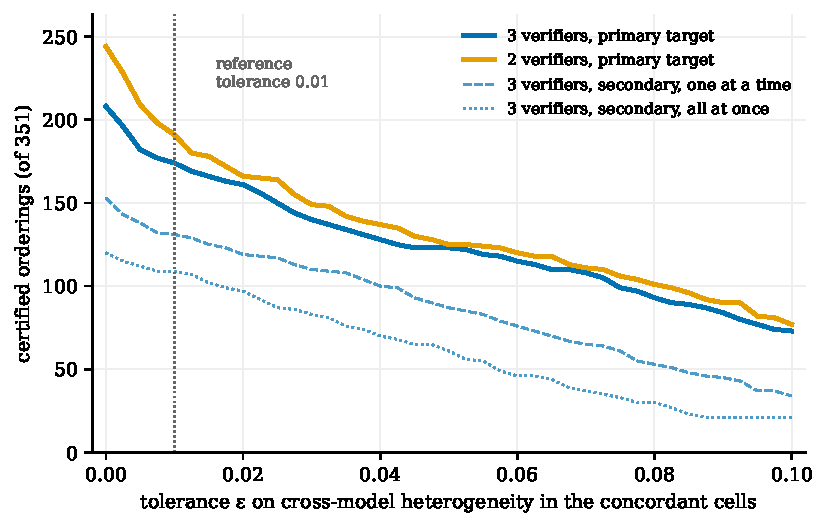
\includegraphics[width=0.66\textwidth]{figures/f2_certified_vs_eps.pdf}
\caption{The paper's main result: certified orderings as a function of the tolerance $\varepsilon$,
the most that the reader's overrule rate may differ between models where the verifiers agree. Solid
lines are the primary target (these problems, all pairs at once) with three and with two verifiers.
Thin blue lines are the secondary target with three verifiers, one ordering at a time (dashed) and
all at once (dotted). The vertical line marks the reference tolerance.}
\label{fig:eps}
\end{figure}

\begin{figure}[t]
\centering
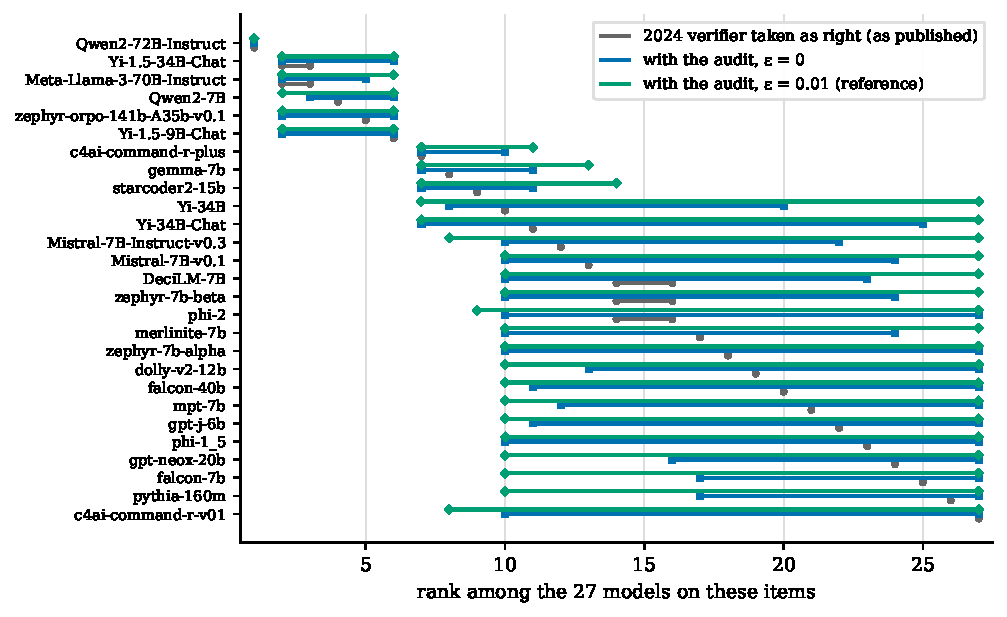
\includegraphics[width=0.92\textwidth]{figures/f1_rank_intervals.pdf}
\caption{Each model's possible ranks on these problems, holding for all orderings at once with
family-wise confidence \FamilyLevelFixed{}. Grey is the ranking the leaderboard prints, which takes its
2024 verifier as right about every response and has no interval except where accuracies tie. Blue
and green are our analysis at $\varepsilon = 0$ and at the reference tolerance. Without sharing
labels between models (not drawn), every model's interval spans all \NumModels{} ranks.}
\label{fig:ranks}
\end{figure}

\section{How many orderings survive}
\label{sec:results}

We now apply the method to the roster. The main answer concerns the \NumItems{} problems the
leaderboard actually used; we then ask what changes if the problems are treated as a sample of
possible questions, and how the answer depends on the verifiers and on our analysis choices.

\subsection{On these problems: the principal result}

Every count in this subsection holds for all \NumOrderings{} orderings at once: the probability that
all of them are right together is at least \FamilyLevelFixed{}, with no large-sample approximation, but only
under Assumption~\ref{ass:h} at the stated $\varepsilon$. With no sharing of labels between models, which assumes nothing about how
the models relate, no ordering is certified: \CertFixedNoPooling{} of \NumOrderings{}. Allowing the
overrule rate to differ between models by at most $\varepsilon = \EpsPrereg$ certifies
\CertFixedPrereg{} orderings, and requiring the models to be exactly alike, $\varepsilon = 0$,
certifies \CertFixedEpsZero{}. The answer to the paper's question is therefore a curve, not a single
number.

Figure~\ref{fig:eps} draws that curve. The certified count falls smoothly as the tolerance grows.
Among the orderings certified at $\varepsilon = 0$, the median breakdown value is
$\varepsilon^* = \BreakdownMedianFixed$, several times the reference tolerance: half of these
orderings would survive that much model-to-model variation in the concordant cells, and half would
not.

Figure~\ref{fig:ranks} shows what this means for someone reading the board. The printed ranking
takes the 2024 verifier as right about every response and gives each model a single rank. Measured
against a human reader, only \RanksResolvedPrereg{} rank is pinned down at the reference tolerance:
the top model keeps first place. The median model's rank is uncertain by \RankWidthMedianEpsZero{}
places at $\varepsilon = 0$ and by \RankWidthMedianPrereg{} at the reference tolerance, and without
shared labels any model could hold any of the \NumModels{} places.

\subsection{Beyond these problems}

A claim about questions like these in general adds the item-sampling term of
Section~\ref{sec:inference}, and the counts fall. Even with the 2024 verifier taken as right about
every response, item sampling alone allows only \CeilingEm{} orderings to be certified one at a time,
which is the ceiling for this target. With the audit, \CertEpsZero{} orderings are certified one at a
time at $\varepsilon = 0$ and \CertPrereg{} at the reference tolerance, and \CertPreregSim{} when
all must hold at once; the distribution-free sampling term certifies \CertHoeffding{} one at a time
at $\varepsilon = 0$. These counts answer a different question at a different confidence level and
are not compared with the primary ones (Appendix Figure~\ref{fig:ranks-general}).

\subsection{How the answer depends on the verifiers and on our choices}

\paragraph{Fewer verifiers certify more, and a fourth changes almost nothing.}
With only the leaderboard's two verifiers, \CertFixedKTwoEpsZero{} orderings are certified at
$\varepsilon = 0$ and \CertFixedKTwoPrereg{} at the reference tolerance, against
\CertFixedEpsZero{} and \CertFixedPrereg{} with three. Dropping the boxed verifier sends the responses
on which only it disagrees back into the concordant cells, where they are pinned down tightly. The
price is a stronger assumption: at $\varepsilon = 0$ the two-verifier analysis is the one whose error
exceeded its nominal level in simulation. Because the three verifiers share machinery, we also added
xFinder \citep{yu2024xfinder}, a fine-tuned language model that returns the answer a response
commits to or declines to give one. Its answers are judged by the same equivalence check as the
reader verdict, so it differs from the other verifiers only in how it extracts. It credits
\XfCredited{} responses and declines on \XfAbstained{}, which score $0$, as an unfound answer does
for the other verifiers (Appendix~\ref{app:data}). With four verifiers the discordant responses grow
from \RowsAnyDisagree{} to \NumDiscordantKFour{}, and the certified count at the reference tolerance
moves from \CertFixedPrereg{} to \CertFixedKFourPrereg{} (\CertFixedKFourPreregRelease{} with
xFinder's other system prompt). The verifiers do rank the models differently: across the four,
\RankChangeModels{} of the \NumModels{} models change rank, one by \RankSpreadMax{} places (Appendix
Table~\ref{tab:models}).

\paragraph{Our own analysis choices move the count by a few orderings at most.}
At the reference tolerance, dropping \textsc{none} and \textsc{contradictory} labels gives
\SensDropFixed{}, Clopper--Pearson intervals give \SensCpFixed{}, judging the copied answer with
Math-Verify instead of the benchmark's check gives \SensMvFixed{}, and string comparison, which also
changes the boxed verifier, gives \SensStringFixed{} (Appendices~\ref{app:sensitivity}
and~\ref{sec:sensitivity}).

\section{How common is this design choice?}
\label{sec:generality}

The results so far concern one roster on one board. Two wider questions can be answered without
new labels: whether the choice of verifier also moves the rest of the board, and whether the
scoring design behind the problem is common elsewhere.

\paragraph{Across the whole board.}
The re-scoring, on \BoardRegradeDate{}, rewrote the results file of a model's run with Math-Verify's
scores and did not generate new responses. We traced every displayed score on the board back to its
results file (Appendix~\ref{app:board}). For the \BoardShiftModels{} models whose displayed score
comes from a file the re-scoring rewrote, and whose earlier version we could read, the file's score
before and after the rewrite compares two verifiers on the same responses. Of the pairs that both
scores order strictly, \BoardShiftDiscordantPct\% reverse, that is, swap places
(Appendix~\ref{app:board} defines the statistic and its treatment of ties), and Kendall's rank
correlation between the two scores, which would be $1$ if they ordered every pair alike, is
$\tau_b = \BoardShiftTau$. Among them, on the \RosterShiftModels{} roster models,
\RosterShiftDiscordantPct\% reverse ($\tau_b = \RosterShiftTau$), so the roster understates how far
the choice of verifier moves the board.

\paragraph{Across evaluation frameworks.}
The design choice at the root of the problem is to score an unreadable response as a wrong
answer. We loaded the task configurations of four evaluation frameworks
\citep{biderman2024lessons, opencompass2026, fourrier2024lighteval, openai2024simpleevals} with
each framework's own loader and classified the scoring path of each generative task. In
\texttt{lm-evaluation-harness}, \LmEvalCoerce{} of \LmEvalGenerative{} generative tasks
(\LmEvalCoercePct\%) match an assumed output format and score a failure to match as incorrect. In OpenCompass the figure is
\OpenCompassCoerce{} of \OpenCompassGenerative{} configurations, in \texttt{lighteval}
\LightevalCoerce{} of \LightevalGenerative{} generative metrics, and in \texttt{simple-evals}
\SimpleEvalsCoerce{} of \SimpleEvalsStringMatch{} string-matching modules (Appendix
Table~\ref{tab:frameworks}). A behavioural check, run on a random sample of
\texttt{lm-evaluation-harness} tasks only, confirmed every classification it could test
(Appendix~\ref{app:frameworks}).

These counts say how many tasks could be affected, not how many rankings change; that depends on
how often real responses escape the extraction rule, which we have measured for one benchmark only.

\section{Related work}
\label{sec:related}

Appendix~\ref{app:related} adds two-phase sampling, verification bias, raters without a gold
standard, uncertainty in rankings, design sensitivity and stratified allocation.

\paragraph{Whether a benchmark measures what it claims.}
BetterBench grades benchmarks against criteria for design, implementation and documentation
\citep{reuel2024betterbench}, a complementary framework asks which evaluative claims a piece of
evidence supports \citep{salaudeen2025measurement}, and retrieval tools find the items in a
benchmark that bear on a particular use \citep{diddee2026benchbrowser}. That work sits upstream of
ours: we take the benchmark and its gold answers as given and ask whether the published ranking is
determined by the pipeline's own outputs, which a valid benchmark does not guarantee.

\paragraph{Configuration moves scores, and extraction is part of the configuration.}
Evaluation results move with prompt formatting \citep{sclar2023quantifying}, with small changes
that reorder leaderboards \citep{alzahrani2024benchmarks}, and with the many settings of a widely
used evaluation harness, answer extraction among them \citep{biderman2024lessons}. The sentence
that the 2024 verifier looks for descends from the convention introduced with
Minerva \citep{lewkowycz2022minerva}, and learned extractors have followed \citep{yu2024xfinder}.
The closest study on the extraction side concerns multiple-choice evaluation, where extraction
methods can disagree with human judgement and produce misleading model comparisons
\citep{molfese2025right}. We study free-form mathematical answers and ask which pairwise
comparisons can be established when no extraction method is taken as correct. Benchmarks of verifier accuracy \citep{li2025verifybench} and
verifiers trained to handle the formats that defeat regular expressions
\citep{liu2025compassverifier} go the other way: rank the verifiers and adopt the best. A better
verifier shrinks the discordant cells but does not settle the responses on which verifiers still
disagree.

\paragraph{Label-efficient evaluation with a proxy.}
Prediction-powered inference combines many machine-generated labels with a small human-labelled
sample to produce valid confidence intervals \citep{angelopoulos2023ppi}, with variants for hybrid
evaluation of language models \citep{fisch2024stratified}, active labelling
\citep{zrnic2024active} and synthetic labels \citep{boyeau2025autoeval}. Two papers target
rankings: \citet{chatzi2024ranking} return rank sets with a coverage guarantee from
pairwise comparisons by a strong model calibrated against human comparisons, and
\citet{lee2026judge} correct the bias that a judge's imperfect sensitivity and specificity
introduce into a score. Correcting a proxy's bias requires its error characteristics to carry over
to the models being scored; when they are common to all of them,
Proposition~\ref{prop:oneverifier} applies and no pair can be reversed relative to another. We
therefore bound instead of correcting, with homogeneity assumed only where verifiers with different
extraction rules agree and carried as a parameter that we vary. The cost is fewer conclusions,
each conditional on a tolerance a reader may dispute.

\paragraph{Partial identification and design sensitivity.}
The bounds of Section~\ref{sec:setup} are partial-identification statements
\citep{manski2003partial}, closest to classical results on contaminated data
\citep{horowitz1995identification} and on binary variables misclassified at unknown rates
\citep{molinari2008partial}, with the models as sub-populations. Concurrent
work applies partial identification to the prevalence of a latent attribute reported by a panel of
language models, calibrated against validation labels \citep{chen2026partial}; Appendix~\ref{app:related}
states how our design differs.

\section{Limitations}
\label{sec:limitations}

\begin{enumerate}
\item \emph{The pooling assumption is not tested.} Testing it model by model needs labels drawn
  by model within the concordant cells, which the 400-item audit, stratified otherwise, does not
  provide, and the reference tolerance is a judgement, not calibrated against any external study
  (Section~\ref{sec:setup}). If the
  assumption fails at that tolerance, the certified counts are too high, which is why every result
  is reported as a curve over $\varepsilon$, with a breakdown value for each ordering and the
  no-pooling analysis beside it.
\item \emph{The reader verdict inherits the benchmark's reference solutions.} Every verifier and
  the reader verdict grade against the same reference solutions: the harness derives its gold
  answer from each solution's last boxed expression, and re-deriving it agrees on
  \GoldConsistentN{} of \NumItems{} items; a normalisation rule that damages \GoldFtItems{} of those
  answers changes no audited verdict (Appendix~\ref{sec:sensitivity}). An error in a reference solution therefore affects our
  results and the leaderboard's in the same way, and no analysis inside the pipeline can detect it.
  An audit of a sample of reference solutions would.
\item \emph{The verifiers share machinery.} A response that defeats the shared symbolic library
  could be miscounted by all three verifiers and land in a concordant cell, which would hide
  disagreement rather than create it. xFinder, which extracts differently, moved the count by one.
\item \emph{The scope is one benchmark on one archived board.} The roster of \NumModels{} models
  is a convenience sample that sits low on the board and moved less than the board under the
  change of verifier, so its counts are unlikely to overstate the problem but do not estimate it;
  the secondary analysis also treats a curated benchmark as a random sample.
\item \emph{The labels come mainly from one labeller, the author.} On overlaps of \LabTwoN{} and
  \LabThreeN{} items, two others agree with the reader verdicts in \LabTwoPct\% and \LabThreePct\%
  of cases, and the labels carry no record of the time spent on each item (Appendix~\ref{app:data}).
\end{enumerate}

\section{Conclusion}
\label{sec:conclusion}

A leaderboard names the model but not the verifier, and on this roster the choice of verifier
moves the ranking without the published score showing it. A small human audit can settle part of
the ranking, but only under an explicit assumption about how models differ where the verifiers
agree. Without that assumption this audit certifies \CertFixedNoPooling{} of the \NumOrderings{}
orderings on these problems; at the reference tolerance it certifies \CertFixedPrereg{}, all at once
and with a finite-sample guarantee. The honest output is the curve between the two, with a breakdown
value for every ordering.

Most disagreements here were responses in which a verifier found no answer. Publishing, beside
each score, the verifier, its version and that count, which the pipeline computes and then
discards, would let a reader bound how far a score could rise if every unread response were correct.
It would not settle the disagreements that remain after extraction, which only a reader can. The
assumption this paper rests on can be tested directly with labels drawn model by model in the
concordant cells, and that is the natural next step.


\bibliographystyle{tmlr}
\bibliography{references}

\appendix

\section*{Reproducibility}

Every number in this paper is computed by released code from released result files. The
\SuppName{} holds the code, the verifier configurations, every verifier's verdict on
every response, the human labels, our analysis plan with its dated amendments, and the 400-item
audit's design document.

\section{Proofs}
\label{app:proofs}

Throughout this appendix a concordant cell $c$ is partitioned into sub-populations indexed by
$g$, where a sub-population is a model, or a model crossed with a design stratum when the
audit design was stratified more finely inside the cell. Sub-population $g$ contains $N_{gc}$
responses, of which a fraction $p_{gc}$ has reader verdict $Y^* = 1$. The audit draws
$n_{gc}$ of them by simple random sampling without replacement, independently across $g$, and
observes $x_{gc}$ responses with $Y^* = 1$ among those drawn. We write
$n_c = \sum_g n_{gc}$, $x_c = \sum_g x_{gc}$, $w_{gc} = n_{gc}/n_c$,
$\hat p_c = x_c / n_c$ and $\tilde p_c = \sum_g w_{gc}\, p_{gc}$, and
$\mathrm{KL}(a \,\|\, b) = a \log(a/b) + (1-a)\log\bigl((1-a)/(1-b)\bigr)$ for
$a, b \in [0,1]$, with the conventions $0 \log(0/b) = 0$ and $a \log(a/0) = +\infty$ for $a > 0$.
Thus $\mathrm{KL}(a \,\|\, b) = +\infty$ when $b \in \{0, 1\}$ and $a \ne b$, and
$\mathrm{KL}(1 \,\|\, b) = -\log b$. We assume $n_c \ge 1$; a cell without labels is given the interval
$[0,1]$.

Two remarks come before the proofs. The estimand $\tilde p_c$ is the
\emph{design-weighted} mean of the sub-population rates, not the population mean of cell $c$.
Those coincide when the audit samples each sub-population in proportion to its size, and they
do not in general. And $\tilde p_c$ is a quantity the design defines; the certification result
uses it only through the interval $[L_c, U_c]$, together with
Assumption~\ref{ass:h}, which ties every $p_{gc}$ to every other.

\paragraph{Random label counts.}
The setup above treats each $n_{gc}$ as fixed. A design that samples by model and cell fixes them;
the 400-item audit does not. It was stratified on the
boxed verifier's verdict and the subject, so the number of its labels that land in a given
sub-population of a given three-verifier cell is random. The lemma still applies, by
conditioning. Take $g$ to be a model crossed with a design stratum. Within one stratum the
audit draws a uniformly random subset of fixed size, and conditional on how many of the drawn
responses fall in each (sub-population, cell) domain of that stratum, the responses drawn from
each domain form a uniformly random subset of that domain of the realised size, independently
across domains: the uniform distribution over subsets with given domain counts factorises into
a product of uniform distributions, one per domain. Strata are drawn independently. Hence,
conditional on the realised vector of counts $\{n_{gc}\}$, the $x_{gc}$ are independent
hypergeometric counts exactly as the lemma assumes, and its bound holds with $\tilde p_c$
formed from the realised weights. Because the bound holds for every realisation of the counts,
the coverage statement below holds unconditionally, for a target that is itself random through
its weights. Proposition~\ref{prop:range} is unaffected, since it needs $\tilde p_c$ only to be
some convex combination of the sub-population rates, which it is for every realisation. The
test suite checks this case directly, by simulating an audit stratified on a variable other
than the cell (Appendix~\ref{app:tests}).

\subsection{Proof of Lemma~\ref{lem:kl}}

\begin{proof}[Proof of Lemma~\ref{lem:kl}]
Each $x_{gc}$ is the number of responses with $Y^* = 1$ in a simple random sample without
replacement of size $n_{gc}$ from a population of $N_{gc}$ responses of which $N_{gc}p_{gc}$
have $Y^* = 1$, so $x_{gc}$ is hypergeometric. The argument has four steps.

\emph{Step one: sampling without replacement is dominated.} Theorem~4 of
\citet{hoeffding1963probability} states that if $X_1, \dots, X_n$ is a sample drawn without
replacement from a finite population and $Y_1, \dots, Y_n$ is a sample of the same size drawn
with replacement from the same population, then
$\mathbb{E}\, f\bigl(\sum_i X_i\bigr) \le \mathbb{E}\, f\bigl(\sum_i Y_i\bigr)$ for every
continuous convex $f$. Take $f(z) = e^{\lambda z}$, which is convex for every real $\lambda$.
The with-replacement sum is binomial, so
\[
\mathbb{E}\, e^{\lambda x_{gc}} \;\le\; \bigl(1 - p_{gc} + p_{gc} e^{\lambda}\bigr)^{n_{gc}} .
\]
The inequality goes in the direction we need for both tails, because it holds for negative
$\lambda$ as well as positive.

\emph{Step two: the strata multiply.} The $G$ samples are drawn independently, so the moment
generating function of $x_c$ is the product of the individual ones:
$\mathbb{E}\, e^{\lambda x_c} \le \prod_g (1 - p_{gc} + p_{gc}e^{\lambda})^{n_{gc}}$.

\emph{Step three: heterogeneous rates are dominated by their weighted mean.} Let
$\varphi(p) = \log\bigl(1 + p(e^{\lambda} - 1)\bigr)$, so that the product above is
$\exp\bigl(\sum_g n_{gc}\,\varphi(p_{gc})\bigr)$. Writing $u = e^{\lambda} - 1$,
\[
\varphi''(p) \;=\; \frac{-u^2}{(1 + pu)^2} \;\le\; 0 ,
\]
so $\varphi$ is concave on $[0,1]$ for every $\lambda$. Jensen's inequality with the weights
$w_{gc}$, which are nonnegative and sum to one, gives
$\sum_g w_{gc}\, \varphi(p_{gc}) \le \varphi\bigl(\sum_g w_{gc}\,p_{gc}\bigr) = \varphi(\tilde p_c)$.
Multiplying by $n_c$ and exponentiating,
\[
\mathbb{E}\, e^{\lambda x_c} \;\le\; \bigl(1 - \tilde p_c + \tilde p_c e^{\lambda}\bigr)^{n_c} .
\]
The heterogeneity has been absorbed: the bound is now the moment generating function of a
single binomial at the weighted mean rate.

\emph{Step four: Chernoff, including the boundary cases.} Fix $t$ with
$0 < t \le 1 - \tilde p_c$; for larger $t$ the event $\{\hat p_c \ge \tilde p_c + t\}$ is empty, and
when $\tilde p_c = 1$ no $t$ is admissible, so there is nothing to prove. For
every $\lambda > 0$, Markov's inequality applied to $e^{\lambda x_c}$ gives
\[
\Pr\bigl(\hat p_c \ge \tilde p_c + t\bigr)
\;\le\; \exp\Bigl( -\lambda n_c (\tilde p_c + t) + n_c \log\bigl(1 - \tilde p_c + \tilde p_c e^{\lambda}\bigr) \Bigr) ,
\]
so the probability is at most the infimum of the right side over $\lambda > 0$. Three cases
cover every admissible $t$. If $\tilde p_c = 0$, every sub-population that carries labels has
$p_{gc} = 0$, so $x_c = 0$ with certainty and the probability is
$0 = e^{-n_c \mathrm{KL}(t \,\|\, 0)}$. If $\tilde p_c > 0$ and $\tilde p_c + t < 1$, the exponent is
minimised at
$e^{\lambda^{\star}} = \frac{(\tilde p_c + t)(1 - \tilde p_c)}{(1 - \tilde p_c - t)\,\tilde p_c}$,
which is finite and larger than one, and substituting it gives the exponent
$-n_c\,\mathrm{KL}(\tilde p_c + t \,\|\, \tilde p_c)$. If $\tilde p_c + t = 1$, the event is
$\{x_c = n_c\}$ and the right side equals $\bigl(\tilde p_c + (1 - \tilde p_c)e^{-\lambda}\bigr)^{n_c}$,
which decreases to $\tilde p_c^{\,n_c} = e^{-n_c \mathrm{KL}(1 \,\|\, \tilde p_c)}$ as
$\lambda \to \infty$; the infimum is not attained, and no finite $\lambda^{\star}$ exists or is
needed. This is the first inequality. For the
second, with $0 < t \le \tilde p_c$, apply the same four steps to the complementary counts
$n_{gc} - x_{gc}$, whose rates are $1 - p_{gc}$ and whose weighted mean is $1 - \tilde p_c$, and use
the identity $\mathrm{KL}(1-a \,\|\, 1-b) = \mathrm{KL}(a \,\|\, b)$, which also holds under the
conventions above.
\end{proof}

\paragraph{The interval, and its coverage.}
Inverting the lemma gives the interval used in the paper. Define
\[
[L_c, U_c] \;=\; \bigl\{ q \in [0,1] \;:\; n_c\,\mathrm{KL}(\hat p_c \,\|\, q) \le \log(2/\alpha) \bigr\} ,
\]
which is an interval containing $\hat p_c$, because $q \mapsto \mathrm{KL}(\hat p_c \,\|\, q)$
is convex with its minimum at $q = \hat p_c$.

\begin{proof}[Coverage of the interval]
Consider the event $\{\tilde p_c < L_c\}$. Since $[L_c, U_c]$ contains $\hat p_c$, on this event
$\hat p_c > \tilde p_c$ and $n_c \mathrm{KL}(\hat p_c \,\|\, \tilde p_c) > \log(2/\alpha)$. If
$\tilde p_c = 0$ then $x_c = 0$, so $\hat p_c = 0$ and the event is empty. Otherwise
$a \mapsto \mathrm{KL}(a \,\|\, \tilde p_c)$ is continuous and strictly increasing on
$[\tilde p_c, 1]$, from $0$ to $\mathrm{KL}(1 \,\|\, \tilde p_c)$. If
$n_c \mathrm{KL}(1 \,\|\, \tilde p_c) \le \log(2/\alpha)$, no $\hat p_c \ge \tilde p_c$ can exclude
$\tilde p_c$ and the event is again empty. If not, there is a unique $t^{\star} \in (0, 1 - \tilde p_c)$
with $n_c \mathrm{KL}(\tilde p_c + t^{\star} \,\|\, \tilde p_c) = \log(2/\alpha)$, and the event forces
$\hat p_c > \tilde p_c + t^{\star}$, whose probability is at most $\alpha/2$ by
Lemma~\ref{lem:kl}. The event $\{\tilde p_c > U_c\}$ is bounded by $\alpha/2$ symmetrically,
and the union bound gives coverage at least $1 - \alpha$.
\end{proof}

Nothing in either argument requires the sub-population rates to be equal, requires sampling
with replacement, or appeals to a limit. One check is exact. When no audited response in the
cell has $Y^* = 1$, $\hat p_c = 0$ and
$\mathrm{KL}(0 \,\|\, q) = -\log(1-q)$, so the upper endpoint solves
$-n_c\log(1 - U_c) = \log(2/\alpha)$, giving $U_c = 1 - (\alpha/2)^{1/n_c}$. That is exactly
the Clopper--Pearson upper limit at zero successes \citep{clopper1934use}, so at the boundary
the design-valid interval is no wider than Clopper--Pearson; it is wider only in the interior.

\subsection{Proof of Proposition~\ref{prop:range}}

The proof has three parts: the region contains the truth, the optimisation separates across
cells, and the cellwise optimum has a closed form. For a concordant cell with shares
$a = s_{jc}$ and $b = s_{kc}$, the minimum of $a x - b y$ over $R_c(\varepsilon)$ is
\begin{equation}
a\ell_c - b\min(h_c, \ell_c + \varepsilon) \ \text{ when } a \ge b, \qquad
a\max(\ell_c, h_c - \varepsilon) - b h_c \ \text{ otherwise},
\label{eq:closedform}
\end{equation}
which is what the implementation computes. A fourth part says where the region is sharp and
where it is not.

\begin{proof}[The region contains the truth]
Fix a concordant cell $c$. Model $m$'s rate in that cell is the size-weighted mean of the
rates of the sub-populations belonging to $m$,
$p_{mc} = \sum_{g \in m} (N_{gc}/N_{mc})\, p_{gc}$, and $\tilde p_c$ is the design-weighted
mean $\sum_g w_{gc}\, p_{gc}$ over all of them. Both are convex combinations of the same
numbers $\{p_{gc}\}$. Under Assumption~\ref{ass:h} those numbers lie in a common interval $I$
of width at most $\varepsilon$, and a convex combination of points of $I$ lies in $I$.
Therefore $p_{jc}$, $p_{kc}$ and $\tilde p_c$ all lie in $I$, which gives
$|p_{jc} - p_{kc}| \le \varepsilon$ and $|p_{mc} - \tilde p_c| \le \varepsilon$ for
$m \in \{j,k\}$. On the event $\tilde p_c \in [L_c, U_c]$ the second of these yields
$p_{mc} \in [L_c - \varepsilon,\, U_c + \varepsilon]$, and since $p_{mc}$ is a proportion it
also lies in $[0,1]$, so $p_{mc} \in [\ell_c, h_c]$. Together these are exactly the
constraints defining $R_c(\varepsilon)$.
\end{proof}

\begin{proof}[Separability]
By Equation~\eqref{eq:accuracy}, $\Delta_{jk} = \sum_c (s_{jc} p_{jc} - s_{kc} p_{kc})$ is
linear in the unknowns and the shares are known. The constraint set is a product across
cells: each concordant cell contributes $R_c(\varepsilon)$, and each discordant cell
contributes the rectangle $[l_{jc}, u_{jc}] \times [l_{kc}, u_{kc}]$, which is
$[0,1]^2$ when that cell carries no labels for those models. Minimising or maximising a sum of
terms over a product of sets is done term by term. For a discordant cell the optimum is at a
corner, giving $s_{jc} l_{jc} - s_{kc} u_{kc}$ and $s_{jc} u_{jc} - s_{kc} l_{kc}$.
\end{proof}

\begin{proof}[The closed form]
Write $a = s_{jc} \ge 0$, $b = s_{kc} \ge 0$, $\ell = \ell_c$, $h = h_c$, and minimise
$f(x,y) = a x - b y$ over
$R = \{(x,y) \in [\ell,h]^2 : |x - y| \le \varepsilon\}$.

For fixed $x \in [\ell,h]$, the objective decreases in $y$, so the optimal $y$ is the largest
feasible one, $y = \min(h,\, x + \varepsilon)$. This is feasible: it is at most $h$ by
construction, at least $\ell$ because $x \ge \ell$ and $h \ge \ell$, and within $\varepsilon$
of $x$ because it is at most $x + \varepsilon$ and at least $\min(h,x) = x$. Substituting,
\[
g(x) \;=\; a x - b \min(h,\, x + \varepsilon)
\;=\;
\begin{cases}
(a - b)\,x - b\,\varepsilon, & x \le h - \varepsilon, \\
a\,x - b\,h, & x \ge h - \varepsilon,
\end{cases}
\]
a piecewise linear function whose slope rises from $a - b$ to $a$ at the kink
$x = h - \varepsilon$. Since $b \ge 0$ the slope is nondecreasing, so $g$ is convex.

If $a \ge b$, both slopes are nonnegative and $g$ is nondecreasing, so the minimum is at
$x = \ell$ and equals $a\ell - b\min(h, \ell + \varepsilon)$.

If $a < b$, the first slope is negative and the second is nonnegative, so the unconstrained
minimiser is the kink, and the constrained minimiser is $x^{\star} = \max(\ell,\, h -
\varepsilon)$. When $h - \varepsilon \ge \ell$ the value is $a(h-\varepsilon) - bh$. When
$h - \varepsilon < \ell$ the minimiser is $\ell$, and since then $\ell + \varepsilon > h$ the
value is $a\ell - bh$. Both cases are written by the single expression
$a\max(\ell,\, h - \varepsilon) - b\,h$.

The maximum follows by symmetry. $R$ is invariant under exchanging its two coordinates, and
$\max_R (a x - b y) = -\min_R (b x - a y)$ after that exchange, so the maximum is obtained by
applying the formula above with $a$ and $b$ swapped and negating the result.
\end{proof}

\begin{proof}[Sharp at $\varepsilon = 0$, conservative above it]
At $\varepsilon = 0$ we have $\ell_c = L_c$ and $h_c = U_c$, and $R_c(0)$ is the diagonal
segment $\{(q,q) : q \in [L_c, U_c]\}$. Every point of it is attained in the relaxation where
each $p_{gc}$ may take any value in $[0,1]$: set every sub-population rate in the cell to $q$,
which satisfies $H(0)$ and makes $p_{jc} = p_{kc} = \tilde p_c = q$. The interval for
$\Delta_{jk}$ is therefore attained and cannot be narrowed, which is what sharpness means
here. The qualification about the relaxation matters, because each $p_{gc}$ is really a
fraction over finitely many responses and only finitely many values of $q$ are exactly
attainable. This is the same granularity that Section~\ref{sec:setup} uses to argue that
$H(0)$ is an idealisation rather than a hypothesis about the world.

For $\varepsilon > 0$ the region is an outer bound, and the reason is that it forgets the
weights. $R_c(\varepsilon)$ imposes only that $p_{jc}$ and $p_{kc}$ lie within $\varepsilon$
of each other inside $[\ell_c, h_c]$. The actual constraint is stronger: the same
sub-population rates that produce $p_{jc}$ and $p_{kc}$ must also produce a design-weighted
mean $\tilde p_c$ lying in $[L_c, U_c]$. When one model supplies most of the audit weight in
the cell, its own rate is pinned close to $\tilde p_c$ and cannot travel the full distance
$\varepsilon$ away from $[L_c,U_c]$. The computed range therefore contains the sharp
identified range. Every consequence runs in the safe direction: reported ranges are at least
as wide as the truth requires, fewer orderings are certified than a sharp analysis would
certify, and each breakdown value in Definition~\ref{def:breakdown} is a lower bound on the
sharp one.
\end{proof}

\subsection{Proof of Proposition~\ref{prop:oneverifier}}

\begin{proof}[Proof of Proposition~\ref{prop:oneverifier}]
Let $a_m$ be the fraction of model $m$'s responses the single verifier credits. Conditioning
on the verifier's verdict and using the assumed common predictive values,
\[
A_m \;=\; \Pr(Y^\ast = 1 \mid v = 1)\, a_m + \Pr(Y^\ast = 1 \mid v = 0)\,(1 - a_m)
\;=\; \pi_0 + a_m (\pi_1 - \pi_0),
\]
so $\Delta_{jk} = A_j - A_k = (\pi_1 - \pi_0)(a_j - a_k)$.
\end{proof}

The same statement in the other natural parameterisation makes the consequence easier to see.
Suppose instead that the verifier has common error rates, $q = \Pr(v = 1 \mid Y^\ast = 0)$ and
$r = \Pr(v = 0 \mid Y^\ast = 1)$, shared by all models. Then
$a_m = (1-r) A_m + q (1 - A_m) = q + (1 - q - r) A_m$, so
$a_j - a_k = (1 - q - r)\,\Delta_{jk}$. The observed gap is the gap under the reader verdict,
scaled by one number.

Either way, a single multiplicative constant relates every observed pairwise gap to the
corresponding gap under the reader verdict. Three consequences follow, and they are the reason the design uses
more than one verifier.

The sign of every pairwise comparison is determined by the sign of that constant. When
$\pi_1 > \pi_0$, equivalently $q + r < 1$, every ordering the verifier reports is the ordering
under the reader verdict. When $\pi_1 < \pi_0$ every ordering is reversed at once. A model that a common
mechanism treats unusually badly does not exist inside this parameterisation.

Pair-specific reversals are therefore outside the model. A reversal that affects one pair and
leaves another intact cannot be produced by any choice of $\pi_0$ and $\pi_1$, so observing
one is evidence that the mechanism differs across models. Section~\ref{sec:generality} reports
such reversals.

At $\pi_1 = \pi_0$, equivalently $q + r = 1$, every $\Delta_{jk}$ is zero and the verifier
carries no information about the ordering at all.

The role this plays in the design is the following. Pooling under a single verifier is
Assumption~\ref{ass:h} at $\varepsilon = 0$ with $K = 1$, where the pooled cells cover the
entire population and nothing is left model-specific. That assumption does not merely
simplify the analysis; by the proposition it removes the phenomenon the paper is about. With
$K$ verifiers the pooling is confined to the cells where they agree, and the cells where they
disagree, which is where the disputed responses live, stay model-specific by construction.

\subsection{Proof of Proposition~\ref{prop:coverage}}

\begin{proof}[The audit half, in finite samples]
List the parameters a certification uses: the pooled rate $\tilde p_c$ for each concordant
cell, which is shared by every pair on the roster, and the per-model rate $p_{mc}$ for each
audited discordant cell. Distinct parameters are estimated from disjoint sets of labels, and
conditional on the realised number of labels in every domain those sets are independent (the
paragraph on random label counts above), so the corresponding intervals are conditionally
independent; the argument below is conditional on those counts, and it holds for every
realisation of them. Give each of the $P$ parameters an interval at level
$1 - \alpha'$ with $\alpha' = 1 - (1 - \alpha_{\mathrm{audit}})^{1/P}$, which is the
allocation of \citet{sidak1967rectangular} and is exact rather than conservative under
independence. By Lemma~\ref{lem:kl} each interval covers its parameter with probability at
least $1 - \alpha'$, and by independence all of them cover simultaneously with probability at
least $(1-\alpha')^{P} = 1 - \alpha_{\mathrm{audit}}$.

On that event, the hypothesis of Proposition~\ref{prop:range} holds for every cell at once, so
the identified range computed for every pair contains the corresponding $\Delta_{jk}$
simultaneously. Any ordering whose range lies strictly above zero is therefore correct. No
step used a limit, so the statement is exact in finite samples.
\end{proof}

\begin{proof}[The item-sampling half, asymptotically]
Let $\delta_{jk}$ denote the pairwise difference over the distribution from which the
benchmark's items were drawn, and $\Delta_{jk}$ the difference on the realised items. With
$D_i$ the difference of the two models' reader verdicts on item $i$, the sample mean
of $D$ is $\Delta_{jk}$ and its expectation is $\delta_{jk}$. The central limit theorem gives
$\Pr(|\delta_{jk} - \Delta_{jk}| > z_{1-\alpha_s/2}\sqrt{\mathrm{Var}(D)/N}) \to \alpha_s$,
and replacing $\mathrm{Var}(D)$ by the upper bound of Section~\ref{sec:inference} can only
widen the interval. Combining the two halves by a union bound,
\[
\Pr\bigl(\delta_{jk} \notin [\mathrm{LB}_{jk} - h_{jk},\, \mathrm{UB}_{jk} + h_{jk}]\bigr)
\;\le\; \Pr\bigl(\Delta_{jk} \notin [\mathrm{LB}_{jk}, \mathrm{UB}_{jk}]\bigr) + \Pr\bigl(|\delta_{jk} - \Delta_{jk}| > h_{jk}\bigr) ,
\]
which is at most $\alpha_{\mathrm{audit}} + \alpha_{\mathrm{sample}}$. The two events concern
different sources of error, one the labels and the other the items, so nothing is counted
twice; adding the levels rather than convolving the two error distributions is what makes the
combination conservative.
\end{proof}

For a family of orderings, the audit half is already simultaneous because the concordant
intervals are shared and the discordant allocation runs over all audited per-model parameters.
The sampling half is made simultaneous by a Bonferroni division of $\alpha_{\mathrm{sample}}$
across the family. Rank intervals inherit the family level directly: on the event that every
certified ordering is correct, at least one model is ranked above $m$ for each ordering
$k \succ m$ that was certified and at least one below for each $m \succ k$, so $m$'s true rank
lies between one plus the first count and the number of models less the second.

\subsection{The paired variance bound}
\label{app:paired}

Section~\ref{sec:inference} bounds the item-sampling variance without observing the reader
verdict on unaudited items. Two elementary steps do the work.

First, $D_i$ takes values in $\{-1,0,1\}$, so $D_i^2$ is the indicator that the two models are
scored differently and $\mathrm{Var}(D) \le \mathbb{E}[D^2] = \Pr(D \ne 0)$.

Second, for any verifier $v$ and any response pair,
\[
\mathbf{1}[Y^\ast_j \ne Y^\ast_k] \;\le\; \mathbf{1}[v_j \ne v_k] + \mathbf{1}[Y^\ast_j \ne v_j] + \mathbf{1}[Y^\ast_k \ne v_k] .
\]
If the left side is one and all three terms on the right are zero, then $v_j = v_k$,
$Y^\ast_j = v_j$ and $Y^\ast_k = v_k$, which forces $Y^\ast_j = Y^\ast_k$ and contradicts the
left side. Averaging over items, the disagreement rate between the two models under the reader
verdict is at most the verifier's own disagreement rate between them, which is observed on
every item, plus each model's disagreement rate with that verifier, which the identified
bounds of Proposition~\ref{prop:range} bound above at the same $\varepsilon$. Taking the
smallest bound over the available verifiers, and capping at one, gives the quantity used in
the half-width. It is paired, because the verifier disagreement term is computed item by item
rather than from the two models' marginal accuracies, and it is conservative, because every
ingredient is an upper bound.

\section{Numerical checks of the stated results}
\label{app:tests}

Appendix~\ref{app:proofs} proves the results. This appendix describes what is checked
numerically, which is a different question with three parts: whether the code computes what
the propositions say, whether the prose says what the code computes, and whether a change to
the data pipeline silently moves a number that was fixed earlier. The released test suite holds
\TestsTotal{} cases in \TestsFunctions{} test functions.

\subsection{The propositions against independent computation}

The first group of tests, \TestsCertification{} cases, compares the implementation with
computations that do not share its code path.

The closed form of Proposition~\ref{prop:range} is checked against brute force on randomly
drawn cells: a dense grid over $R_c(\varepsilon)$, together with the region's exact polygon
vertices so that an optimum sitting between grid points cannot be missed. A separate check
asserts where the minimiser sits, not only what the minimum equals, because a formula can
return the right value from the wrong argument and stay wrong at the next input. Three
degenerate configurations are pinned explicitly: the cell where no verifier credits, in which
$L_c = 0$ and the clipping binds for every positive $\varepsilon$; a cell in which both
models have zero share and must contribute nothing; and an $\varepsilon$ large enough that the
region is the whole unit square.

Monotonicity of the lower bound in $\varepsilon$ is checked over a grid, since
Definition~\ref{def:breakdown} is well posed only if it holds. The breakdown value itself is
checked by running the bisection and, separately, scanning a fine grid for the first
$\varepsilon$ at which the margin fails; the two must agree to a stated tolerance. The
interior slope of a concordant cell's contribution is checked to be
$-\max(s_{jc}, s_{kc})$, which rules out the valid but looser slope $-(s_{jc} + s_{kc})$; the
looser slope would pass every other check.

Proposition~\ref{prop:oneverifier} is checked in both parameterisations over random draws,
for every pair in a synthetic board, which is the form in which the claim is actually used:
not that some pair is scaled, but that all of them are scaled by the same number. The claim
that sampling without replacement can only help is checked against exact binomial coefficients
rather than against the bound that replaces them.

Lemma~\ref{lem:kl} gets four checks. At zero and at full successes the interval must equal
the Clopper--Pearson limit exactly, which is the boundary identity derived in
Appendix~\ref{app:proofs}. The interval must contain the point estimate and must widen with
the level. A Monte Carlo draws pooled hypergeometric samples from sub-populations with
deliberately different rates and requires the realised miss rate not to exceed nominal; that
check exercises both departures the lemma is about at once, and it is the one that would fail
if the Jensen step were wrong. A second Monte Carlo stratifies the draw on a variable other
than the cell, so that the number of labels in each domain is random, and requires the interval
to cover the mean formed with the realised weights, which is the conditioning argument of
Appendix~\ref{app:proofs}. A last check compares both tail bounds with exact probabilities at the
boundaries treated in step four ($\tilde p_c = 0$, $t = 1 - \tilde p_c$ and $t = \tilde p_c$), and
confirms coverage in the case where no $t^{\star}$ exists; doubling the exponent of the bound makes
it fail.

The level allocation is checked separately: the number of parameters a statement relies on is
computed from one function for a single ordering and for the whole roster, with and without
pooling, and a test confirms that an allocation over one pair's parameters falls short of the
stated family-wise level once per-model discordant intervals exist.

Rank intervals are checked against a small board whose certified set and correct answer are
written out by hand.

\subsection{The printed formulas against the implementation}

Transcription is where errors enter a paper, so a second group of tests,
\TestsManuscriptClaims{} cases, re-implements the formulas exactly as printed here, without
importing the library, and compares them with the implementation on random inputs. It covers
the closed form~\eqref{eq:closedform}, Proposition~\ref{prop:oneverifier}, the claim that
$\varepsilon = 0$ collapses to the pooled analysis, and the claim that certification is
monotone. A formula changed in the paper but not in the code, or the reverse, makes these tests
fail.

\subsection{The regression anchor}

A third group, \TestsAnchor{} cases, rebuilds the earlier seventeen-model, two-verifier
configuration from the \emph{current} verdicts and audit map and requires it to reproduce the
counts that the earlier two-verifier pipeline produced under its string semantics:
\AnchorStringCombined{} orderings for the secondary target and \AnchorStringAudit{} for the
primary target, one ordering at a time. Its purpose is to catch any change to the verdicts, the
audit map or the verifiers that silently alters a previously reported result, which is the
class of failure the defect of Section~\ref{sec:data} belongs to.

\subsection{What these checks do not establish}

They do not prove the propositions; Appendix~\ref{app:proofs} does. They do not validate the
empirical results, which come from the released result files. And a check written from the same misunderstanding as the code will pass. That is the
reason for the division of labour above: the propositions are proved on paper, the
second group re-implements from the printed text rather than from the library, and
the anchor compares against numbers fixed before the current code existed.

\section{Inference details}
\label{app:inference}

\subsection{How the levels are allocated}

The audit and the item sample are controlled separately, at $\alpha_{\mathrm{audit}} =
\AlphaAudit$ and $\alpha_{\mathrm{sample}} = \AlphaSample$, and a claim that generalises
beyond the benchmark's items is made at one minus their sum. Proposition~\ref{prop:coverage}
is what licenses adding them.

Within the audit, the level is divided across the parameters a claim uses, by the allocation
$\alpha' = 1 - (1-\alpha_{\mathrm{audit}})^{1/P}$. For a single ordering those parameters are
the pooled interval of each concordant cell, plus each of the two models' per-model
discordant intervals. For a statement about every ordering at once they are every parameter on
the roster: the pooled intervals, which every pair shares, plus every per-model discordant
interval, each of which enters every ordering its model appears in. Both kinds of statement
count parameters the same way, and a test checks that a per-pair count would fall short of the
stated family-wise level.

In the configuration reported here no discordant cell contributes a parameter, because the
400-item audit was not drawn by model and cell; its labels in a discordant cell are described in
Appendix~\ref{app:data} and do not enter the certification. $P$ is therefore the number of
concordant cells for both kinds of statement, every pooled interval is constructed at level
\SidakTwoLevel{}, and the audit side of a family-wide statement is simultaneous without
further widening. The family-wide setting therefore changes only the sampling term, which
takes a Bonferroni division of $\alpha_{\mathrm{sample}}$ across the \NumOrderings{}
orderings. An audit that supplied per-model discordant labels would add parameters, and the audit
intervals of a family-wide statement would widen with them.

Without pooling, each model's concordant intervals enter as model-specific parameters, so a
statement about every ordering at once allocates over two per model on the roster rather than
four per pair. The variance bound in the sampling term is always computed from the same
intervals as the range it widens.

Rank intervals are read off the certified set and inherit whichever level that set was
constructed at, since they are a deterministic function of it.

\subsection{The item-sampling term, for the secondary target}

Under the item-sampling interpretation, a claim about which model is better in general carries
a second source of uncertainty that the audit cannot reduce. We bound it by a paired argument.
For a pair of models, let $D_i$ be the difference of their reader verdicts on item $i$. Then $\mathrm{Var}(D) \le \Pr(D \neq 0)$, and $\Pr(D \neq 0)$ is bounded above by the
observed rate at which a verifier's verdicts differ between the two models, plus each model's
maximum possible disagreement with that verifier, both of which the identified range already
supplies (Appendix~\ref{app:paired}). The resulting half-width is paired, so it exploits the
fact that both models answer the same items, and it is conservative, because it uses upper
bounds rather than estimates. It rests on a central limit approximation, so the combined
interval is asymptotic, not exact.

The two sources of error are combined by a union bound, and they are distinct. The audit
interval concerns the unknown correctness rates given these responses; the item-sampling term
concerns generalisation beyond these items. Nothing is counted twice. The two halves of
Proposition~\ref{prop:coverage} are accordingly different in kind: the first is a finite-sample
guarantee that follows from Lemma~\ref{lem:kl}, and the second inherits the central limit
approximation of the sampling term. Rank intervals are reported as the family-level object,
because a reader looking at a leaderboard is reading all the orderings at once, not one.

\subsection{A sampling term that does not rest on a limit}

The paired half-width above is conservative in its variance but asymptotic in its
distribution, and a reader who declines the central limit approximation needs a number, not a
caveat. Because the paired difference $D_i$ lies in
$[-1, 1]$, Hoeffding's inequality bounds the deviation of its mean without any variance
estimate at all, giving the half-width
\[
h \;=\; \sqrt{\frac{2 \log(2/\alpha_{\mathrm{sample}})}{N}} ,
\]
which is finite-sample, distribution-free, and the same for every pair. It is also much
wider, and the cost is visible: for the secondary target, one ordering at a time at
$\varepsilon = 0$, substituting it certifies \CertHoeffding{} orderings where the paired
asymptotic term certifies \CertEpsZero{}. Both are reported: the distribution-free count stands
without the approximation, and the gap between the two is what the approximation buys. The
primary target needs neither, because it carries no sampling term.

\begin{figure}[t]
\centering
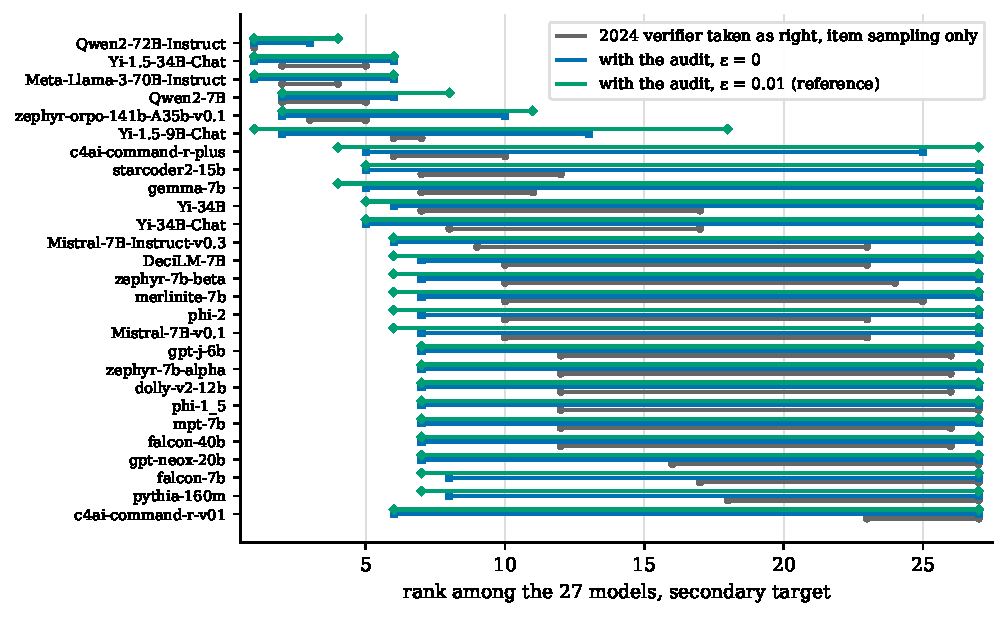
\includegraphics[width=\textwidth]{figures/f5_rank_intervals_generalising.pdf}
\caption{Rank intervals for the secondary target, which also allows for the items being a
sample of possible questions, holding for all orderings at once at an asymptotic level. Grey takes
the 2024 verifier as correct and allows only for item sampling. Without pooling across models (not
drawn), every model's interval spans all \NumModels{} ranks. Compare Figure~\ref{fig:ranks}, which
is the primary target on these items.}
\label{fig:ranks-general}
\end{figure}

The pairing matters separately from the distributional question. An unpaired term, built
from each model's marginal accuracy under one verifier, is kept only to reproduce the
regression anchor of Appendix~\ref{app:tests}; it certifies
\CertSamplingLegacy{} orderings. It is not used, because two models answering the same items
differ on far fewer of them than their marginal accuracies suggest, and a term that ignores
the pairing throws that away.

\subsection{What the coverage simulation does}

The simulation runs \SimScenarios{} scenarios at \SimReplicates{} replicates each, at the full
scale of the roster. It checks whether the guarantee is attained and how it degrades; it is not
a proof.

The frame is the full set of real responses, with the real cell structure and the real audit allocation, so
that the strata, their sizes and their sampling rates are the ones the paper actually uses.
What must be invented is the reader verdict on unaudited responses, and it is invented in two
deliberately different ways.

In the first, each concordant sub-population is given a number of errors that makes the
realised error fractions span an interval of width exactly $\varepsilon_{\mathrm{true}}$, so
that Assumption~\ref{ass:h} holds exactly as a statement about finite populations. This is the
validity check: the procedure is analysed at the same $\varepsilon$, and no certified claim
should be wrong.

In the second, concordant errors are drawn independently with a small propensity that is the
same for every model. No model differs from any other in expectation, which is the most
favourable situation pooling could hope for, and yet the realised fractions differ by chance,
so $H(0)$ fails as a statement about the finite populations that actually exist. This is a
diagnostic rather than a validity check, and it is the one that produced the paper's reason
for not reporting $\varepsilon = 0$ as a result.

Discordant cells are given independent per-model rates drawn uniformly, which is the worst
case the analysis is built for and the reason those cells enter at $[0,1]$ when unaudited.
Items are resampled from the frame with replacement and paired across models, so the
item-sampling term has something real to cover. An audit-only claim is scored against the
difference on the realised items; a combined claim is scored against the superpopulation
expectation. Confusing those two would make the procedure look better than it is, which is why
they are kept apart in the output.

One number bounds what the simulation can resolve. At the nominal level and this many
replicates, the Monte Carlo standard error of a family-wise error rate is \SimMcSeAudit{}, so
a reported rate of zero means below resolution rather than exactly zero, and the scenarios are
compared against nominal with that in mind. Zero failures in \SimReplicates{} replicates is
likewise not a zero error probability: it bounds the family-wise error rate below
\SimZeroFwerUpper{} at \SimZeroFwerConfPct\% confidence, one-sided, so the procedure is
consistent with its stated level and conservative rather than tight.

The second construction is the one that separates the two configurations reported in
Section~\ref{sec:inference}. With equal underlying rates analysed at $\varepsilon = 0$, the
two-verifier analysis exceeds its nominal level and the three-verifier analysis does not, so
exact homogeneity is safe in one configuration and unsafe in the other. Equal underlying rates
do not imply equal realised fractions, so $H(0)$ can fail in the world most favourable to pooling,
which is why the paper does not lead with it.

\section{Sensitivity analyses}
\label{app:sensitivity}

Each analysis in this appendix re-runs the whole pipeline with a single element replaced rather
than recomputing the headline numbers a different way. All but the last row of
Table~\ref{tab:sensitivity} are sensitivity analyses named in our analysis plan; the others it
names are the two-verifier analysis (Section~\ref{sec:results}) and the alternative sampling terms
(Appendix~\ref{app:inference}). The table reports them, with the pooled audit counts each
configuration produces alongside the orderings it certifies, because the counts are what the
certification is downstream of and reporting only the certified number would hide where a
movement came from.

% Generated by scripts/fb_tables_tmlr.py -- do not edit by hand.
\begin{table}[t]
\centering
\caption{Sensitivity analyses. Each row re-runs the whole pipeline with one element of the analysis replaced, and reports the pooled audit counts it produces in the two concordant cells together with the certified orderings, first for the primary target (all orderings at once) and then for the secondary target (one ordering at a time). $^{a}$The pooled interval, in place of Lemma~\ref{lem:kl}. $^{b}$The routine that decides $Y^*$. $^{c}$\textsc{none} and \textsc{contradictory} excluded rather than scored incorrect. $^{d}$Changes the boxed verifier \emph{and} the equivalence routine, so cells move too. $^{e}$A different set of models: its counts are out of a smaller family and are not comparable down the column.}
\label{tab:sensitivity}
\small
\begin{tabular}{lccrrrr}
\toprule
& & & \multicolumn{2}{c}{primary target} & \multicolumn{2}{c}{secondary target} \\
\cmidrule(lr){4-5}\cmidrule(lr){6-7}
analysis & $111$ & $000$ & $\varepsilon=0$ & $\varepsilon=\EpsPrereg$ & $\varepsilon=0$ & $\varepsilon=\EpsPrereg$ \\
\midrule
primary analysis & 142/144 & 0/223 & 208 & 174 & 153 & 131 \\
Clopper--Pearson interval$^{a}$ & 142/144 & 0/223 & 209 & 174 & 155 & 131 \\
Math-Verify equivalence$^{b}$ & 141/144 & 1/223 & 206 & 172 & 143 & 128 \\
indeterminates dropped$^{c}$ & 142/144 & 0/186 & 207 & 174 & 152 & 130 \\
string semantics$^{d}$ & 141/142 & 0/223 & 196 & 168 & 141 & 127 \\
seventeen-model subset$^{e}$ & 142/143 & 0/145 & 99 & 89 & 76 & 68 \\
\bottomrule
\end{tabular}
\end{table}


Four features of the table matter.

The primary result is stable. On these items at the reference tolerance, every alternative
that keeps the verifiers fixed lands within a few orderings of \CertFixedPrereg{}. The choice of
interval makes no difference there at all: Clopper--Pearson, which is tighter but exact only
under assumptions this design does not satisfy, also certifies \SensCpFixed{}. The headline does
not depend on having used the conservative interval, so the conservative one is used because it
is the valid one here, not because the result needs it.

The secondary result moves more, and mostly for one reason. Judging the reader's transcription
with Math-Verify costs the primary target a handful of orderings and the secondary target many
more;
Appendix~\ref{sec:sensitivity} explains why the same labels matter so differently to the two.

The string-semantics row moves both targets furthest, but it changes a verifier as well as the
equivalence routine, so it is not a clean test of either.

The last row is a different question from the others. It restricts the roster to a
seventeen-model subset, so its counts are out of \NumOrderingsSeventeen{} orderings rather than
\NumOrderings{} and cannot be compared down the column. It is in the table because it is the
configuration the regression anchor of Appendix~\ref{app:tests} reproduces.

What none of these rows do is vary Assumption~\ref{ass:h}. They vary the analysis applied to
a fixed assumption. The assumption itself is varied by the $\varepsilon$ curve of
Figure~\ref{fig:eps} and summarised per ordering by the breakdown value, and that is the
sensitivity analysis the paper is actually built around. The rows here answer the narrower
question of whether a defensible alternative choice inside the pipeline would have produced a
different story, and none of them does.

\section{Sensitivity to the equivalence routine and to indeterminate answers}
\label{sec:sensitivity}

Section~\ref{sec:data} defines the reader verdict in two steps, and only the first is human. A
labeller transcribes the final answer a response commits to, and an equivalence routine then
compares that transcription with the benchmark's gold answer; $Y^*$ is whatever the routine
returns. The routine is a choice, and since this paper is about scoring choices that go
unreported, ours is reported here.

The primary analysis uses the benchmark harness's own routine, the same symbolic comparison the
leaderboard applies to its gold answers. We use it because the question is whether a response
would have been credited had a reader, rather than an extraction rule, decided what it says, and
holding the equivalence step at the benchmark's own routine isolates the extraction step, which
is the thing under study. It is not necessarily the best routine available.

\paragraph{A different equivalence routine.}
Deciding $Y^*$ with Math-Verify instead credits \SensMvCorrectRejectAll{} audited response in
the cell where no verifier credits, against \AuditCorrectRejectAll{} under the harness routine,
and \SensMvCorrectAgreeAll{} of \AuditNAgreeAll{} in the cell where all three credit, against
\AuditCorrectAgreeAll{}. Both differences push the bounds the same way. On these items the
certified count moves from \CertFixedEpsZero{} to \SensMvFixedEpsZero{} at $\varepsilon = 0$,
and from \CertFixedPrereg{} to \SensMvFixed{} at the reference tolerance. For the secondary
target it moves from \CertEpsZero{} to \SensMvCombined{} at
$\varepsilon = 0$, one ordering at a time.

The same two labels matter very differently to the two targets, and the reason shows where the
pipeline is fragile. The cell where no verifier credits holds \CellRejectAll{} responses, and
one audited response with reader verdict $1$ raises the upper end of its interval substantially. In the identified range of a pairwise difference, that
interval enters multiplied by the \emph{difference} between the two models' shares of the cell,
which is usually small, because most of every model's responses land there; so the primary
target barely moves. In the sampling term of the secondary target, the same interval enters each model's own
bound on its disagreement with a verifier, multiplied by that model's \emph{own} share, which is
close to one, and the two models' bounds add. That is where most of the secondary target's
movement comes from. The equivalence routine is therefore a minor choice for the primary claim
and a consequential one for the secondary claim.

\paragraph{String comparison.}
The third row of the same family is reported in Table~\ref{tab:sensitivity} and should be read
with care, because it is not a one-factor change. The boxed verifier and the equivalence routine
share a normalisation and comparison implementation, so switching to string comparison
changes which cell a response falls into as well as how its transcription is judged. The
label counts move accordingly: the cell where all three verifiers credit holds
\SensStringNAgreeAll{} audited responses rather than \AuditNAgreeAll{}. On these items at the
reference tolerance certification falls to \SensStringFixed{}; for the secondary target at
$\varepsilon = 0$ it falls to \SensStringCombined{}. We report the row because string
comparison is what the defective
verifier of Section~\ref{sec:data} actually computed, and we do not attribute the movement to
the equivalence routine alone.

\paragraph{Responses with no answer, and responses with two.}
A labeller who finds no final answer records \textsc{none}, and one who finds two answers both
presented as final records \textsc{contradictory}. The primary analysis counts both as
incorrect. The alternative is to drop them, which reduces the audited labels in the cell where
no verifier credits from \AuditNRejectAll{} to \SensDropNRejectAll{}. On these items at the
reference tolerance the certified count stays at \SensDropFixed{}; for the secondary target
at $\varepsilon = 0$ it moves from \CertEpsZero{} to \SensDropCombined{}.

The two agree closely for a mechanical reason.
Dropping the indeterminates removes labels without removing any credited response, so the
numerator stays at its floor while the denominator shrinks; the interval widens slightly and
nothing else moves. The choice would matter more in a cell where indeterminate responses were
a large share of the credited ones, and the design does not guarantee that they never are.

The reason the primary analysis counts them as incorrect is not statistical convenience. Every
verifier in the pipeline scores a response with no extractable final answer as zero, and the
comparison the paper is making is against what the leaderboard reports. Dropping such
responses would compare against a quantity no leaderboard computes, so Section~\ref{sec:data}
makes this choice part of the definition of the reader verdict.

\paragraph{A normalisation rule that edits gold answers.}
The harness normaliser deletes every occurrence of the letters ``ft'' (feet), including inside
LaTeX commands, so \texttt{\textbackslash infty} becomes \texttt{\textbackslash iny} and
\texttt{\textbackslash left} becomes \texttt{\textbackslash le}, and the harness applied it to the
gold answers when it built the dataset; a public discussion of the leaderboard's archive reports
the resulting damage \citep{oll2026discussion}. Normalising each reference solution's boxed answer
with and without the rule, we find \GoldFtItems{} affected items, the number the discussion
reports, and on each the stored answer is the damaged one. The rule is also applied to every transcription, so the reader verdict
compares like with like, but we checked rather than assumed: \GoldFtLabels{} audited labels fall on
these items, \GoldFtConcordant{} of them in a concordant cell, and recomputing their reader verdicts
without the rule changes \GoldFtChanged{} of them. Every certified count is therefore unchanged.

\paragraph{What none of this settles.}
Every row above holds the benchmark's gold answers fixed. An error in a gold answer propagates
identically through the primary analysis and through all of its alternatives, and no
sensitivity analysis run inside the pipeline can detect it. It is the largest thing this design
does not check (Section~\ref{sec:limitations}).

\section{Data, verifiers, and the human audit in detail}
\label{app:data}

\paragraph{How the roster came about.}
By the maintainers' count, the February 2025 re-scoring covered all \BoardModelsRescored{} models
submitted to the leaderboard up to then \citep{kydlicek2025fixing}. An earlier study catalogued all \RosterCatalogued{} of the
leaderboard's per-model result repositories, ranked them by download count, and kept the top
\RosterSelected{} subject to at most \RosterMaxPerOrg{} per organisation, under a rule written
down before any re-scoring; the cap spread the selection over \RosterOrgs{} organisations. A
download sweep over those models was interrupted, and the \RosterScored{} whose downloads
completed were scored. The 400-item audit drew its items from those, and the
roster is the \NumModels{} that received at least one audited item. Every roster model lies
within the first \RosterDeepestRank{} of the download ranking. Against the leaderboard's final
public table, dated \BoardFinalTableDate{}, which lists \BoardModelsFinal{} models with a MATH-Hard
score because submissions continued after the re-scoring,
\RosterBottomQuartile{} of the \NumModels{} fall in the bottom quartile of displayed accuracy
and \RosterTopQuartile{} in the top. The record behind each count is released with its
checksums. A prespecified rule covered missing responses before the data were assembled, and it
did not fire.

\paragraph{The verifiers' provenance.}
The maintainers described the 2024 verifier as unable to extract answers written
in boxed notation and reported that the re-scoring reordered the top of the board
\citep{kydlicek2025fixing}. From the re-scoring on, the leaderboard displayed scores from one
verifier and published item-level verdicts from another. Table~\ref{tab:provenance} gives the
version, a checksum and the check behind every source the analysis rests on, including the
re-execution that reproduces all \EmReexecItems{} published verdicts.

% Generated by scripts/fb_provenance_table.py -- do not edit by hand.
\begin{table}[t]
\centering
\caption{Provenance of every source the analysis rests on. Hashes are the first twelve hexadecimal digits of the sha256 of the file in the release, with line endings normalised; a dash marks an upstream artefact identified by its pinned version instead. Verifier environment: sympy 1.13.1, latex2sympy2\_extended 1.11.0.}
\label{tab:provenance}
\small
\begin{tabular}{p{0.16\textwidth}p{0.3\textwidth}lp{0.3\textwidth}}
\toprule
artefact & version & hash & check \\
\midrule
published responses & 27 per-model result repositories, 189 subject files; revision of each file recorded in the release & \texttt{--} & sample files unmodified since 2024 in 27 of 27 models \\
2024 verifier & lm-evaluation-harness \texttt{3c8db1bb7b} & \texttt{59604119822c} & re-execution reproduces 35{,}748 of 35{,}748 published verdicts \\
Math-Verify & math-verify 0.9.0 via lm-evaluation-harness \texttt{61ee867816} & \texttt{--} & reproduces the re-scored aggregate in 168 of 175 model-subject combinations \\
boxed verifier & lm-evaluation-harness helpers, in the released code & \texttt{ac7865eec34c} & brute-force and printed-formula tests (Appendix~\ref{app:tests}) \\
xFinder & \texttt{IAAR-Shanghai/\allowbreak xFinder-qwen1505} & \texttt{--} & extractions judged by the equivalence routine \\
scores before re-scoring & \texttt{open-llm-leaderboard/\allowbreak results} at \texttt{c6b22601e3} & \texttt{--} & last revision before February 2025 \\
scores after re-scoring & \texttt{open-llm-leaderboard/\allowbreak contents} at \texttt{9c09a7cae4} & \texttt{--} & final revision of the public table \\
all verifier verdicts & released verdict file & \texttt{878751536bfd} & regenerated by the released pipeline \\
\bottomrule
\end{tabular}
\end{table}


% Generated by scripts/fb_tables_tmlr.py -- do not edit by hand.
\begin{table}[t]
\centering
\caption{What the three verifiers share and where they differ. All three rest on the same symbolic algebra library, and the 2024 and boxed verifiers also share the harness's normalisation and the dataset's gold-answer field. Their agreement is informative because their extraction rules and parsers differ, not because they are independent.}
\label{tab:shared}
\begin{tabular}{llll}
\toprule
step & 2024 verifier & boxed verifier & Math-Verify \\
\midrule
answer extraction & sentence pattern & last boxed expression & LaTeX and expression parse \\
normalisation & harness routine & harness routine & latex2sympy2 \\
equivalence & sympy & string, then sympy & Math-Verify \\
gold answer & dataset field & dataset field & parsed from the solution \\
\bottomrule
\end{tabular}
\end{table}


\paragraph{The fourth verifier and its sixteen cells.}
xFinder reads each response and returns an answer or an abstention. An extraction that is empty
or reads ``no valid answer'' (ignoring case, brackets and parentheses) is an abstention and
receives verdict $0$, as does an extraction whose comparison with the gold answer is stopped after
sixty seconds; every other extraction is judged by the equivalence routine that decides the reader
verdict. Appending xFinder's verdict to the three-verifier string gives sixteen cells, of which
\KFourCellsOccupied{} are occupied. The concordant cells are $0000$ and $1111$, and
Assumption~\ref{ass:h} applies to them; the other fourteen are discordant and enter each model's
range at $[0,1]$, as the three-verifier discordant cells do. Every audited response in a three-verifier concordant cell stays concordant
(\KFourAuditNAgreeAll{} labels in $1111$, \KFourAuditNRejectAll{} in $0000$), so the pooled
intervals are unchanged, and the four-verifier count moves only because \KFourMovedFromConcordant{}
responses leave the concordant cells where xFinder disagrees with the other three. The primary
arm uses the system prompt the extractor was fine-tuned with; the other uses its shipped
default.

\paragraph{The defect in our own verifier.}
While tracing where each verdict came from, we found that the boxed verifier had been silently
degraded. Its symbolic comparison guards itself with a timer that exists only on Unix; on Windows
the guard raised an exception, a broad error handler swallowed it, and every comparison returned
``not equivalent'', so every verdict was in effect a string comparison. Correcting it changes the
number of responses on which it disagrees with the 2024 verifier, on a seventeen-model subset kept
as a regression anchor, from \DisagreeSbEmSeventeenString{} to \DisagreeSbEmSeventeen{}. All
results use the corrected verifier. Correcting it also changes the secondary-target certified count on the
seventeen-model regression anchor (Appendix~\ref{app:tests}), one ordering at a time, from
\AnchorStringCombined{} to \AnchorSympyCombined{}. The anchor is the only configuration in which
both versions can be computed on the same labels.

\paragraph{The 400-item audit's discordant labels.}
Some of the 400-item audit's labels land in a discordant cell: \AuditDiscLabels{} of them, all in
one cell, spread over \AuditDiscModels{} models at a median of \AuditDiscMedianPerModel{} per
model. A discordant cell enters the identified range only through a per-model interval, and the
analysis takes those intervals only from labels drawn by model and cell, which these are not. They
therefore appear in Table~\ref{tab:cells} and Figure~\ref{fig:cells} but not in the certified
counts.

\begin{figure}[t]
\centering
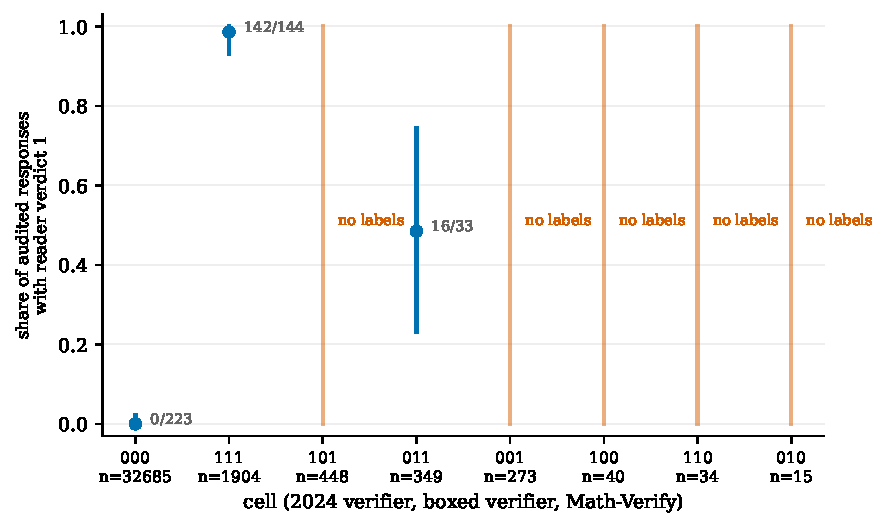
\includegraphics[width=\cellfig]{figures/f3_correctness_by_cell.pdf}
\caption{Share of audited responses in each cell with reader verdict $1$, that is, whose
transcribed answer the benchmark's equivalence routine accepts. Intervals are from
Lemma~\ref{lem:kl}. Five cells carry no labels in the 400-item audit and are bounded only by
$[0,1]$; the labelled discordant cell is shown for description
and does not enter the certification.}
\label{fig:cells}
\end{figure}

\paragraph{How reliable the 400-item audit's labels are.}
The author labelled all 400 items. A second labeller labelled an overlap of \LabTwoN{} of them
and a third a nested overlap of \LabThreeN{}, with both overlaps drawn before any label was seen; each was shown the problem and the response and nothing else. Scoring the
transcribed answers with the equivalence routine, the first and second labellers agree on
\StrOneTwoPct\% of the overlap (Cohen's $\kappa = \StrOneTwoKappa$), the first and third on
\StrOneThreePct\% ($\kappa = \StrOneThreeKappa$), and the second and third on \StrTwoThreePct\%
($\kappa = \StrTwoThreeKappa$). What enters the certification is the reader verdict $Y^*$, and
on it the second labeller agrees with the first on \LabTwoAgree{} of \LabTwoN{} items
($\kappa = \LabTwoKappa$) and the third on \LabThreeAgree{} of \LabThreeN{} ($\kappa =
\LabThreeKappa$). The disagreements are not in the cells that carry the result. In the cell where
no verifier credits there are none (\LabTwoZeroN{} and \LabThreeZeroN{} overlapping labels), and in
the cell where all three credit there are \LabTwoAllDis{} of \LabTwoAllN{} and \LabThreeAllDis{} of
\LabThreeAllN{}; the others fall in discordant cells, which do not enter the counts. Replacing the
first labeller's labels on the overlap by the second labeller's moves the certified count at the
reference tolerance from \CertFixedPrereg{} to \LabSwapTwoPrereg{} (from \CertFixedEpsZero{} to
\LabSwapTwoEpsZero{} at $\varepsilon = 0$), and replacing them by the third's leaves it at
\LabSwapThreePrereg{}. The overlaps are subsets of the 400 items, so this bounds the sensitivity
to the labeller on those subsets only. The audit was labelled in a spreadsheet, so its labels carry no
record of the time spent on each item.

\paragraph{What was fixed, and when.}
Table~\ref{tab:chronology} lists each analysis choice with the document that fixed
it and whether the 400-item audit's labels already existed at the time. Only the audit's design
came before its labels. This study's analysis plan, written for the larger audit before any of that
audit's labels existed, came after the 400-item audit's labels, and so did everything it fixes:
the method of this paper, the tolerance and the sensitivity analyses. The choice of primary target
came later still, after the audit's results for both targets were known. The analysis reported here should therefore be read as
designed with those labels in hand. What protects it from tuning is that every count is reported
as a curve over $\varepsilon$, beside the analysis without pooling, and both targets in full. The
\SuppShort{} holds both documents with their dates.

\begin{table}[h]
\centering
\caption{When each analysis choice was fixed, relative to the 400-item audit's labels.}
\label{tab:chronology}
\small
\begin{tabular}{>{\raggedright\arraybackslash}p{\chronwide}>{\raggedright\arraybackslash}p{\chronmid}>{\raggedright\arraybackslash}p{\chronlast}}
\toprule
choice & fixed in & the audit's labels \\
\midrule
design of the 400-item audit & design document of the earlier study & not yet collected \\
the method: cells, pooled intervals, level allocation & this study's analysis plan and its first four amendments & already existed \\
tolerance $\varepsilon = \EpsPrereg$ and the sensitivity analyses & fourth amendment & already existed \\
fixed-item target as primary & sixth amendment & existed, with results for both targets known \\
larger audit by model and cell, and the discordant census & fourth and sixth amendments & not labelled; no result uses them \\
\bottomrule
\end{tabular}
\end{table}

\section{The roster against the board}
\label{app:board}

Figure~\ref{fig:board-position} places the roster in the distribution of displayed MATH-Hard
accuracy over every model in the leaderboard's final public table (\BoardFinalTableDate{}), and
Figure~\ref{fig:board-shift} plots each traced model's score under the 2024 verifier against its
score under Math-Verify, both read from the same results file. Both use the leaderboard's own
records at fixed revisions; neither involves re-scoring by us. The roster sits low on the board,
and it moved less under the change of verifier than the board did.

\paragraph{Tracing each displayed score.}
The re-scoring rewrote results files in each model's details repository on \BoardRegradeDate{},
changing the MATH-Hard scores and their task version; in every roster file we could compare, the
run's configuration was left unchanged (Table~\ref{tab:provenance}). For each of the \BoardBothModels{} models with a MATH-Hard score both
in the results revision of \BoardPreRescoreDate{} and in the final public table, we listed the
results files in its details repository with the date of the last change to each, read every file
changed on the re-scoring day, and compared its MATH-Hard score with the displayed one, taking the
largest when a model is listed at more than one numerical precision. The displayed score equals the
score of a re-scored file for \BoardAttributable{} models. For \BoardNoRegraded{} models no file was
re-scored, for \BoardMismatch{} the displayed score matches none of the re-scored files, and for
\BoardUnavailable{} the repository could not be read. Over every displayed row of the models we could
read, \BoardStaleRows{} rows match no re-scored file, consistent in kind with a public audit that
reports displayed rows left on the old verifier \citep{oll2026discussion}.

\paragraph{The reversal statistic.}
For \BoardShiftModels{} of the traced models we could also read the re-scored file as it stood before
the re-scoring. Let $a_m$ be model $m$'s MATH-Hard score in that file before the re-scoring and
$b_m$ its score in the same file after it, so that both scores come from one run and one set of
responses. The \BoardShiftModels{} models form \BoardShiftPairs{} unordered pairs $\{i, j\}$. A
pair is \emph{reversed} when $(a_i - a_j)(b_i - b_j) < 0$. The reported share divides the number of
reversed pairs, \BoardShiftReversed{}, by the number of pairs that both scores order strictly,
those with $(a_i - a_j)(b_i - b_j) \neq 0$, of which there are \BoardShiftPairsStrict{}. Pairs tied
under either score (\BoardShiftTiedOld{} under the 2024 score and \BoardShiftTiedNew{} under the
re-scored one, with some overlap) enter neither count; counting them as not reversed instead gives
\BoardShiftReversedAllPct\%. On the roster, \RosterShiftReversed{} of the
\RosterShiftPairsStrict{} strictly ordered pairs reverse. Kendall's $\tau_b$ uses its standard
correction for ties.

A simpler comparison pairs each model's score in the results revision of \BoardPreRescoreDate{}
with its displayed score, and over the \BoardBothModels{} models it gives \BoardSnapshotPct\%. It
mixes runs, though: the earlier revision's score is the same run's score before the re-scoring for
only \BoardSnapshotSameRun{} of the \BoardShiftModels{} same-run models. Restricted to the
\BoardAttributable{} models whose displayed score is a re-scored one, it gives
\BoardAttributablePct\%. The three comparisons agree to within a percentage point.

\paragraph{Were the responses the same?}
The same-run comparison holds the run fixed, and the response files themselves were not rewritten.
For the roster every response file in the model's details repository was last changed in 2024
(Table~\ref{tab:provenance}). For the board we drew \BoardDateSampleN{} of the \BoardBothModels{}
models at random with a fixed seed and read the commit history of every MATH-Hard response file in
each model's details repository; in \BoardDateUnchanged{} of the \BoardDateSampleN{}, every such file
was last changed on or before \BoardPreRescoreDate{}. With no exception in the sample, the share of
the board's models whose response files changed is below \BoardDateUpperPct\% at
\BoardDateConfPct\% confidence (exact, one-sided).

\begin{figure}[htbp]
\centering
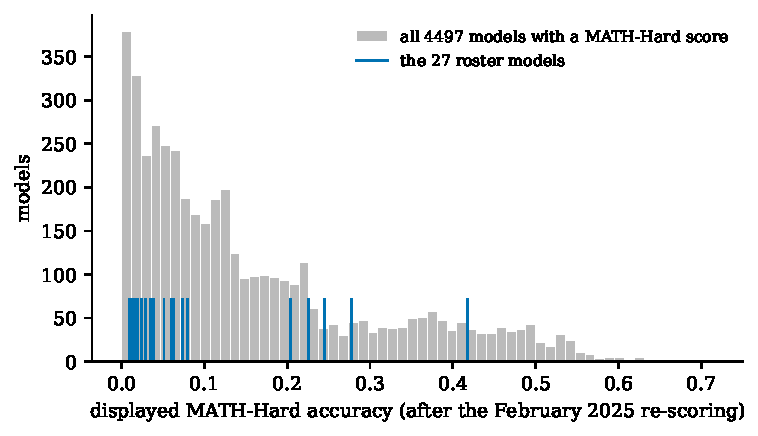
\includegraphics[width=\boardfig]{figures/f6_board_position.pdf}
\caption{Displayed MATH-Hard accuracy after the February 2025 re-scoring, for every model in
the leaderboard's final public table of \BoardFinalTableDate{} (grey), with the roster marked
(blue).}
\label{fig:board-position}
\end{figure}

\begin{figure}[htbp]
\centering
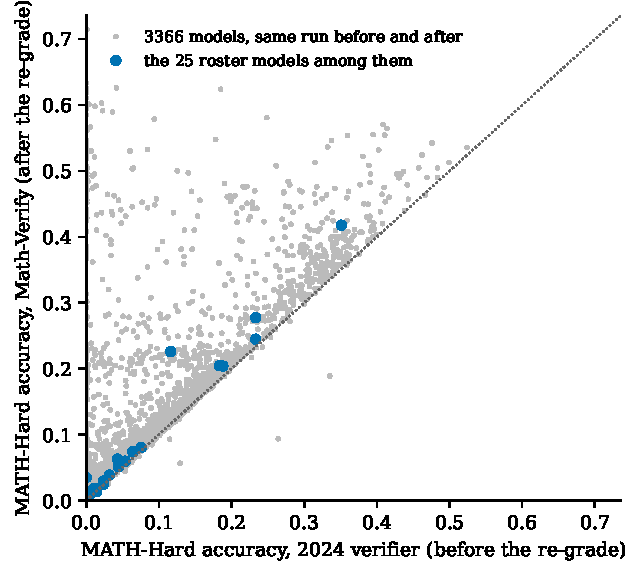
\includegraphics[width=\boardfig]{figures/f8_board_same_run.pdf}
\caption{Each traced model's MATH-Hard accuracy under the 2024 verifier against its accuracy under
Math-Verify, both read from the same results file before and after the re-scoring, for the
\BoardShiftModels{} same-run models; the roster models among them are marked. The responses are
the same on both axes, so points off the diagonal are moved by the verifier alone; the column near
zero on the horizontal axis consists of models whose answers the 2024 verifier could not read.}
\label{fig:board-shift}
\end{figure}

\section{The framework census}
\label{app:frameworks}

% Generated by scripts/fb_tables_tmlr.py -- do not edit by hand.
\begin{table}[t]
\centering
\caption{Scoring configurations that record a failure to extract an answer as an incorrect answer, in four evaluation frameworks at fixed versions. Denominators are different kinds of unit and are not estimates of one common population of tasks. The last column gives, where it was run, the share of sampled units whose behaviour matched their classification, for flagged units and for controls. $^{a}$The version used for the behavioural check; the version used for the classification was not recorded.}
\label{tab:frameworks}
\small
\setlength{\tabcolsep}{3pt}
\begin{tabular}{llrrrl}
\toprule
framework & version & units & flagged & \% & validated \\
\midrule
lm-evaluation-harness & \texttt{f4d4b3de}$^{a}$ & 4{,}524 tasks & 2{,}936 & 64.9 & 93/93 and 100/100 \\
OpenCompass & \texttt{60a28a72} & 1{,}070 configurations & 158 & 14.8 & no \\
lighteval & \texttt{932e1f2f} & 37 metrics & 13 & 35.1 & no \\
simple-evals & \texttt{652c89d0} & 6 string-matching modules & 4 & 66.7 & no \\
\bottomrule
\end{tabular}
\end{table}


Table~\ref{tab:frameworks} summarises the classification of Section~\ref{sec:generality}.
Reading code is not the same as running it, so the classification was validated behaviourally,
for \texttt{lm-evaluation-harness} only; the other three frameworks were classified from their
configurations alone. For a random sample of tasks the declared filter pipeline was rebuilt from the framework's own
classes and run on a well-formed response and on an equivalent response carrying the same
answer in ordinary prose. Of \CensusValidTestable{} testable sampled tasks, all
\CensusValidConfirmed{} behaved as classified, and of \CensusControlN{} control tasks drawn
from the tasks classified as unaffected, all \CensusControlClean{} were confirmed unaffected.

\section{The disagreement taxonomy}
\label{app:gallery}

\paragraph{Template compliance.}
A response is \emph{template compliant} when the 2024 verifier's extraction step finds an answer in
it. That step appends the string ``I hope it is correct.'' to the response and searches the result
(Python's \texttt{re.search}) for the pattern
\texttt{Final Answer: The final answer is(.*?). I hope it is correct.}, whose dots are unescaped
and match any character. The response is compliant when the search succeeds, and the captured
group is the answer the verifier then judges. Compliance is computed for all \NumRows{} responses
with the scoring function recorded in the leaderboard's result files.

\paragraph{The decision tree.}
Every discordant response is classified by the following rules, applied in order; the first rule
that applies decides the class.
\begin{enumerate}
\item \emph{Runtime}: any of the three verifiers timed out or was stopped on the response.
\item \emph{Extraction}: at least one verifier that gave no credit found no answer, meaning that
  the 2024 verifier gave $0$ and the response is not template compliant, the boxed verifier gave
  $0$ and the response contains no \texttt{\textbackslash boxed\{\}}, or Math-Verify gave $0$ and
  could not parse an answer. The sub-class lists every verifier for which this holds (template,
  box, parse, or a combination such as template+box).
\item \emph{Judgement}: otherwise. Every verifier that gave no credit extracted an answer.
\end{enumerate}
The classes are exclusive and cover every discordant response by construction.
Table~\ref{tab:gallery} shows one response of each class, drawn at random with a fixed seed.

% Generated by scripts/fb_extraction_taxonomy.py -- do not edit by hand.
\begin{table}[t]
\centering
\caption{One discordant response per class, drawn at random with a fixed seed rather than chosen, showing its last characters. The cell is the verdict string (2024 verifier, boxed verifier, Math-Verify).}
\label{tab:gallery}
\small
\begin{tabular}{p{0.2\textwidth}cp{0.62\textwidth}}
\toprule
class & cell & end of the response \\
\midrule
extraction: template & 011 & \texttt{\footnotesize fer by that amount.  However, since the order of \$a\$ and \$b\$ does not matter, each pair of polynomials will be counted twice.  Therefore, there are \$\textbackslash{}frac\{12\textbackslash{}cdot2\}\{2\} = \textbackslash{}boxed\{12\}\$ ordered pairs \$(a,b)\$.  The answer is: 12<|im\_start|>user } \\
\addlinespace
extraction: box & 101 & \texttt{\footnotesize ation is accurate, and the answer is well-explained. Good job!   <|im\_start|>\} userNo problem! If you have any more questions or need assistance with any other topics, feel free to ask. I'm here to help!  5The answer is: 5<|im\_start|>\} user} \\
\addlinespace
judgement & 011 & \texttt{\footnotesize g this inequality, we find \$m < -8\$ or \$m > 8\$. Therefore, the possible values of \$m\$ are \$\textbackslash{}boxed\{(-\textbackslash{}infty, -8) \textbackslash{}cup (8, \textbackslash{}infty)\}\$. Final Answer: The final answer is \$(-\textbackslash{}infty, -8) \textbackslash{}cup (8, \textbackslash{}infty)\$. I hope it is correct.  <|im\_start|>user } \\
\addlinespace
\bottomrule
\end{tabular}
\end{table}


\paragraph{By model and by subject.}
Tables~\ref{tab:models} and~\ref{tab:subjects} break the board down further, still without human
labels. The verifiers do not affect every model alike. Template compliance ranges from
\TemplateMinPct\% to \TemplateMaxPct\% of a model's responses, and \RankChangeModels{} of the
\NumModels{} models change rank across the four verifiers. The median change is
\RankSpreadMedian{} place; the largest, \RankSpreadMax{} places, belongs to the model that almost
never writes the template sentence. By Proposition~\ref{prop:oneverifier}, two informative
verifiers whose errors were alike for every model would order every pair the same way, so changes of this kind
show errors that differ across models. By subject, the share of responses in a discordant cell
ranges from \DiscSubjectMinPct\% to \DiscSubjectMaxPct\%, and in every subject most disagreements
are failures to extract, between \ExtrSubjectMinPct\% and \ExtrSubjectMaxPct\% of them, so the
pattern is not confined to one area of the benchmark.

% Generated by scripts/fb_model_subject_table.py -- do not edit by hand.
\begin{table}[t]
\centering
\footnotesize
\caption{Every roster model under each verifier, without human labels; all shares are percentages. Accuracy is the share of the model's responses credited; rank 1 is the highest accuracy among the roster, with ties sharing the best rank, and the spread is the largest minus the smallest of the four ranks. Template is the share of responses in which the 2024 verifier's extraction finds an answer; discordant is the share in a cell where the three verifiers disagree. Rows are in the order of the 2024 verifier.}
\label{tab:models}
\setlength{\tabcolsep}{3pt}
\begin{tabular}{lrrrrcrrr}
\toprule
 & \multicolumn{4}{c}{accuracy} & ranks & & & \\
\cmidrule(lr){2-5}
model & 2024 & boxed & MV & xF & 2024/boxed/MV/xF & spread & template & discordant \\
\midrule
Qwen2-72B-Instruct & 35.1 & 36.6 & 41.7 & 40.6 & 1/1/1/1 & 0 & 83.8 & 8.9 \\
Yi-1.5-34B-Chat & 23.3 & 21.5 & 27.7 & 26.7 & 2/3/2/2 & 1 & 84.8 & 9.2 \\
Meta-Llama-3-70B-Instruct & 23.3 & 24.2 & 24.5 & 24.9 & 2/2/3/3 & 1 & 95.6 & 4.4 \\
Qwen2-7B & 18.8 & 17.7 & 20.4 & 20.4 & 4/5/6/5 & 2 & 94.3 & 5.0 \\
zephyr-orpo-141b-A35b-v0.1 & 18.4 & 14.0 & 20.5 & 20.4 & 5/6/5/5 & 1 & 90.3 & 7.9 \\
Yi-1.5-9B-Chat & 11.6 & 19.6 & 22.6 & 22.2 & 6/4/4/4 & 2 & 45.2 & 12.0 \\
c4ai-command-r-plus & 7.6 & 7.3 & 8.0 & 8.5 & 7/7/7/7 & 0 & 92.4 & 2.3 \\
gemma-7b & 6.4 & 5.6 & 7.5 & 7.4 & 8/8/8/8 & 0 & 75.7 & 3.2 \\
starcoder2-15b & 5.4 & 5.1 & 6.0 & 6.0 & 9/9/10/9 & 1 & 73.3 & 1.7 \\
Yi-34B & 4.5 & 2.7 & 5.1 & 5.1 & 10/11/11/11 & 1 & 69.0 & 3.2 \\
Yi-34B-Chat & 4.3 & 1.7 & 6.3 & 6.0 & 11/16/9/9 & 7 & 55.2 & 5.1 \\
Mistral-7B-Instruct-v0.3 & 3.2 & 2.3 & 3.9 & 3.7 & 12/12/12/12 & 0 & 84.9 & 2.2 \\
Mistral-7B-v0.1 & 2.5 & 1.6 & 2.9 & 2.7 & 13/17/14/14 & 4 & 64.8 & 1.6 \\
DeciLM-7B & 2.4 & 1.9 & 2.8 & 2.6 & 14/13/17/16 & 4 & 65.7 & 1.2 \\
zephyr-7b-beta & 2.4 & 1.8 & 2.9 & 2.6 & 14/15/15/16 & 2 & 83.2 & 1.4 \\
phi-2 & 2.4 & 1.2 & 2.9 & 2.7 & 14/18/15/14 & 4 & 76.6 & 2.2 \\
merlinite-7b & 2.3 & 1.9 & 2.4 & 2.5 & 17/13/18/18 & 5 & 94.4 & 1.1 \\
zephyr-7b-alpha & 1.5 & 0.9 & 2.0 & 1.7 & 18/19/19/19 & 1 & 67.1 & 1.2 \\
dolly-v2-12b & 1.4 & 0.5 & 1.4 & 1.6 & 19/22/24/21 & 5 & 85.8 & 1.1 \\
falcon-40b & 1.4 & 0.8 & 1.8 & 1.7 & 20/20/20/19 & 1 & 65.0 & 1.1 \\
mpt-7b & 1.3 & 0.8 & 1.6 & 1.4 & 21/21/22/22 & 1 & 49.8 & 1.0 \\
gpt-j-6b & 1.2 & 0.5 & 1.4 & 1.4 & 22/23/23/23 & 1 & 42.4 & 1.4 \\
phi-1\_5 & 1.1 & 0.2 & 1.7 & 1.2 & 23/24/21/24 & 3 & 42.1 & 2.0 \\
gpt-neox-20b & 0.6 & 0.2 & 1.4 & 0.9 & 24/26/24/25 & 2 & 39.4 & 1.4 \\
falcon-7b & 0.5 & 0.2 & 1.0 & 0.7 & 25/24/26/26 & 2 & 35.7 & 0.9 \\
pythia-160m & 0.2 & 0.0 & 1.0 & 0.6 & 26/27/26/27 & 1 & 10.8 & 1.0 \\
c4ai-command-r-v01 & 0.0 & 3.2 & 3.5 & 3.5 & 27/10/13/13 & 17 & 0.1 & 3.8 \\
\bottomrule
\end{tabular}
\end{table}

% Generated by scripts/fb_model_subject_table.py -- do not edit by hand.
\begin{table}[t]
\centering
\footnotesize
\caption{The seven MATH-Hard subjects, over all roster responses, without human labels; shares are percentages. Columns as in Table~\ref{tab:models}; extraction is the share of the subject's discordant responses whose disagreement is a failure to extract an answer (Table~\ref{tab:taxonomy}).}
\label{tab:subjects}
\setlength{\tabcolsep}{4pt}
\begin{tabular}{lrrrrrrrr}
\toprule
 & & \multicolumn{4}{c}{accuracy} & & & \\
\cmidrule(lr){3-6}
subject & responses & 2024 & boxed & MV & xF & template & discordant & extraction \\
\midrule
algebra & 8{,}289 & 11.0 & 11.5 & 14.7 & 14.1 & 69.4 & 5.7 & 67.9 \\
intermediate algebra & 7{,}560 & 1.9 & 1.9 & 2.6 & 2.4 & 53.3 & 1.3 & 80.2 \\
prealgebra & 5{,}211 & 13.5 & 11.5 & 15.4 & 15.3 & 75.9 & 5.5 & 88.4 \\
number theory & 4{,}158 & 6.6 & 5.7 & 7.3 & 7.1 & 65.0 & 1.9 & 93.8 \\
precalculus & 3{,}645 & 2.6 & 2.7 & 2.8 & 3.5 & 52.9 & 2.7 & 61.2 \\
geometry & 3{,}564 & 2.8 & 3.0 & 4.0 & 3.6 & 70.5 & 1.7 & 69.4 \\
counting and probability & 3{,}321 & 5.7 & 4.9 & 6.4 & 6.3 & 75.8 & 2.0 & 95.5 \\
\bottomrule
\end{tabular}
\end{table}

\clearpage

\section{Related work in detail}
\label{app:related}

This appendix continues Section~\ref{sec:related} with the comparisons that bear on the design
rather than on the question.

\paragraph{Partial identification with model-generated labels.}
\citet{chen2026partial} study the prevalence of a latent binary attribute when the evidence is a
panel of model reports whose errors may be arbitrarily dependent given the truth. They show that
the prevalence is completely unidentified without restrictions that separate the latent
components, and that weak stochastic-ordering restrictions do not help; identifying power comes
from externally calibrated scores and events, such as reporter accuracy measured on a validation
sample, which they illustrate with a toxicity task that has expert-adjudicated labels. The human
audit in our design plays the role of such a calibration sample. We differ in the target, which
is the difference between models and so an ordering rather than a level; in stratifying by the
agreement of several verifiers, so that the calibration assumption is confined to the cells where
they agree; in carrying the assumption as a parameter $\varepsilon$ with a breakdown value for
each conclusion; and in intervals that are valid under sampling without replacement.

\paragraph{Uncertainty in rankings.}
Rank confidence intervals for language-model leaderboards already exist, built by aggregating
pairwise tests, and recent work examines where their uncertainty comes from on a knowledge
benchmark, in particular variability across subjects \citep{neuhof2026ranking}. That uncertainty is
about which items were asked. The uncertainty here is about how each item was scored, and it
does not shrink as items are added; the secondary analysis of this paper combines the two.

\paragraph{Reporting how far an assumption can be pushed.}
Assumption~\ref{ass:h} is not testable at this budget in any strong sense, so the useful thing to
report is how much of it a conclusion needs. Design sensitivity describes a finding by the
magnitude of unmeasured bias that would be required to explain it away, and compares designs by
how much bias they can tolerate \citep{rosenbaum2004design}; $\varepsilon^{*}_{jk}$ is the amount
of cross-model heterogeneity it would take to overturn $j \succ k$. The analogy also sets the
reporting standard followed here, which attaches the sensitivity parameter to each conclusion as
a number instead of leaving it as a caveat in a discussion section.

\paragraph{Two-phase sampling, verification bias, and raters without a gold standard.}
Two-phase sampling, in which a large first-phase sample is measured cheaply and a small second
phase accurately, goes back to \citet{neyman1938contribution}, and the binomial case with
misclassification, where a fallible classifier is calibrated against a subsample scored by an
infallible one, is \citeauthor{tenenbein1970double}'s double sampling scheme
\citep{tenenbein1970double}. When the subsample is chosen by the fallible classifier's own
verdict, the problem is verification bias, and corrections for it are standard in diagnostic
testing \citep{begg1983assessment}; confidence limits that propagate uncertainty in the
estimated error rates into the corrected prevalence are also available \citep{lang2014confidence}.
Two features of our setting break the classical correction. The reader verdict is observed on a
sample stratified by the agreement pattern of several verifiers rather than by one verifier's
verdict, and the error rates are not assumed common across the populations being compared, which
is the assumption Proposition~\ref{prop:oneverifier} shows to be fatal to the question.

Estimating error rates from several imperfect tests without a gold standard is classical
\citep{hui1980estimating}, as is estimating observer error rates from repeated labels
\citep{dawid1979maximum}. Those methods identify rates by assuming the raters err independently
given the truth. We do not assume that, and Section~\ref{sec:data} reports what the three
verifiers share. Instead of identifying the rates through an independence assumption, we obtain
partial identification from agreement stratification and accept wider intervals.

\paragraph{Where to spend a label budget.}
Deciding how many labels each stratum receives is a stratified sampling problem, and the
classical answer optimises the variance of an estimated mean \citep{neyman1934stratified}, with
unequal selection probabilities handled by the standard weighting
\citep{horvitz1952generalization} and the finite-population corrections used here taken from the
standard texts \citep{cochran1977sampling, kish1965survey}. Adaptive versions that learn the
within-stratum variances while sampling are recent \citep{morikawa2026tsneyman}. An audit designed
for certification faces a different problem. A label can narrow an identified range or test the
assumption on which every certified ordering depends, and the two uses are not commensurable, so
no single variance criterion allocates between them.


\end{document}
